\chapter{Fusão de evidências} \label{cap_fusao}

\section{Método de fusão de evidências de bordas optimal}

Nesta seção serão desenvolvidas as ideias dos artigos \citet{gs} e \citet{fawcett}, baseadas nas propriedades estatísticas do índice Kappa e da curva \textit{Receiver Operating Characteristics} (ROC) aplicadas no contexto de imagens PolSAR.


As curvas ROC são técnicas para visualizar, organizar e selecionar classificadores com base no seu desempenho.   Atualmente temos encontrado a aplicação das curvas ROC em aprendizado de máquina, visão computacional, inteligência artificial entre outras áreas similares demostrando a capacidade deste método para efetuar avaliações e comparações de algoritmos. 

As curvas ROC têm a capacidade de representar satisfatoriamente a compensação entre taxas de acertos e taxas de alarmes falsos dos classificadores tornando-se uma boa ferramente para aplicarmos no presente trabalho. 

Na construção da curva ROC  teremos a tarefa de realizar um problema de classificação com duas classe rotuladas como elementos ou instâncias do conjunto $\{\mathbf{p},\mathbf{n}\}$, onde $\mathbf{p}$ representa a classe positiva e $\mathbf{n}$ representa a classe negativa. O conjunto assim definido será considerado o conjunto com as expectativas verdadeira, ou seja, pode representar a quantidade real de bordas ou não bordas em uma imagem de referência (\textit{ground truth}) ou imagens as quais vamos considerar como imagens de referência.

O processo de classificação pode ser aplicado resultando em uma predição rotulada como $\{\mathbf{P},\mathbf{N}\}$, onde $\mathbf{P}$ é predita positiva e $\mathbf{N}$ é predita negativa. Com as definições anteriores e sendo dado um classificador e um conjunto de instâncias podemos construir uma matriz $2\times 2$, chamada de matriz de confusão (matriz de contingências). 


Definido como as instâncias podem ser classificadas a tabela (\ref{cap_fusao_tab01}) mostra a matriz de confusão.
\begin{itemize}
	\item [-] Se a instância é positiva e classificada como positiva é contada como verdadeiro positivo $TP$;
	\item [-] Se a instância é positiva e classificada como negativa é contada como falso negativo $FN$;
	\item [-] Se a instância é negativa e classificada como negativa é contada como verdadeiro negativo $TN$;
	\item [-] Se a instância é negativa e classificada como positiva é contada como falso positivo $FP$.
\end{itemize}


\begin{table}[hbt]
	\centering
	\caption{Matriz de confusão.}\label{cap_fusao_tab01}
\begin{tabular}{@{}cll@{}} \toprule
	                        & \multicolumn{2}{c}{Classes definidas como verdadeiras}                              \\ \midrule
	 Classes preditas       & $\mathbf{p}$                       & $\mathbf{n}$                        \\
                         $\mathbf{P}$& Verdadeiros Positivos (TP) & Falsos Positivos (FP)      \\ 
	                     $\mathbf{N}$& Falsos Negativos (FN)      & Verdadeiros Negativos (TN) \\ \bottomrule 
\end{tabular}
\end{table}

Os valores da diagonal principal desta matriz representam as classificações realizadas corretamente, enquanto os elementos da diagonal secundária representam a classificação incorreta.
Adicionalmente, observamos que a soma de todas as possibilidades de resultados em uma classificação retorna o valor $1$, isto é, $TP+FN+FP+TN=1$.

No auxílio para a definição de várias métricas vamos definir dois parâmetros usados, respectivamente o parâmetro $P$ é definido como a prevalência, e pode ser calculado por $P=TP+FN$. Podemos afirmar que a prevalência leva em conta os resultados falsos negativos, assim sendo, idealmente a prevalência deveria aproximar-se de $TP$. 
O parâmetro $Q$ , chamado de \textit{Nível-Q} pode ser calculado por $Q=TP+FP$. 
Observando então que o \textit{Nível-Q} leva em conta os resultados falsos positivos, similarmente com a prevalência, 
o \textit{Nível-Q} deveria aproximar-se de $TP$ em situações ideais. 
Analisando a definição do parâmetro \textit{Nível-Q} podemos afirmar que  é uma predição de todos os pixel de bordas, mesmo que sejam uma instância negativa e classificada como positiva. 
Ainda podemos definir $N=FP+TN$, recorrendo ao fato $TP+FN+FP+TN=1$ redefinimos $P+N=1$  

Com as definições de prevalência e \textit{Nível-Q} e as tendências observada podemos afirmar que em um detector de bordas ótimo a prevalência e o \textit{Nível-Q} deveriam ser iguais, isto é, $P=Q$.

A matriz de confusão serve de origem para definirmos métricas como as seguintes:
\begin{equation}\label{cap_fusao_eq_01}
	tp_{rate}=\frac{TP}{P},
\end{equation}
\begin{equation}\label{cap_fusao_eq_02}
	fp_{rate}=\frac{FP}{N}
\end{equation}
as quais serão usada para a construção da curva ROC, a métrica $tp_{rate}$ pode ser chamada por razão de verdadeiros positivos, taxa de acerto, \textit{recall} ou  sensibilidade. 
E a $fp_{rate}$ pode ser chamada por razão de falsos positivos.

Na métrica chamada $recall= tp_{rate}=\frac{TP}{P}=\frac{TP}{TP+FN}$ podemos notar que se o número de falsos negativos tende a zero o \textit{recall} aproxima-se do valor unitário, mostrando o comportamento da métrica com a variação dos falsos negativos.

A precisão $\frac{TP}{Q}=\frac{TP}{TP+FP}$ definida desta forma pode medir uma tendência assintótica para o valor unitário quando os falsos positivos  tende para zero.  

A acurácia $\frac{TP+TN}{P+N}$ definida dessa forma juntamente com o fato de $P+N=1$ resulta que igual a $TP+TN$, nos mostrando uma maneira de estudar a acurácia em relação a tendência de verdadeiros positivos. 
A acurácia é medida pela soma da diagonal principal da matriz de confusão.

As métricas $recall$, precisão e acurácia nos mostram uma maneira de observar os resultados baseados em diferentes propriedades de classificação, respectivamente vamos analisar as métricas com relação aos comportamentos de falsos negativos, falsos positivos e verdadeiros negativos.  

A medida$-F$ pode ser definida e interpretada como, 
\begin{equation}\nonumber
medida-F=\frac{2}{\frac{1}{recall}+\frac{1}{precisao}}
\end{equation}

Realizando manipulações algébricas, seja inicialmente considerando somente o denominador
\begin{equation}\nonumber
	\frac{1}{recall}+\frac{1}{precisao}=\frac{1}{\frac{TP}{Q}}+\frac{1}{\frac{TP}{P}}
\end{equation}
\begin{equation}\nonumber
	\frac{1}{\frac{TP}{Q}}+\frac{1}{\frac{TP}{P}} = \frac{Q+P}{TP}
\end{equation}
logo,
\begin{equation}\nonumber
	medida-F=\frac{2}{\frac{Q+P}{TP}}
\end{equation}
\begin{equation}\nonumber
	medida-F=\frac{2TP}{Q+P}
\end{equation}
e definindo
\begin{equation}\nonumber
     Q+P=2TP+FP+FN
\end{equation}
portanto
\begin{equation}\nonumber
	medida-F=\frac{2TP}{2TP+FP+FN}
\end{equation}
a métrica considera conjuntamente as classificações de $FP$ e $FN$, ou seja, se ambas as métricas tendem para zero, o valor da $medida-F$ tende para $1$. Temos assim uma maneira de observar o comportamento da classificação dependendo dos falsos positivos e falsos negativos.

\section{A curva ROC}
A curva ROC é um gráfico bidimensional no qual o valor de $tp_{rate}$ é imposto no eixo das ordenadas e $fp_{rate}$ será imposto no eixo das abscissas gerando um ponto do gráfico, neste trabalho será gerado um ponto para cada canal considerado. Podemos afirmar que o gráfico gerado descreve uma relação entre as razões de verdadeiros positivos e as razões de falsos positivos. 

Consideraremos um número finito de classificadores vamos gerar uma curva ROC onde cada classificador produz um ponto no espaço da curva ROC, a ser descrito por ($fp_{rate}, tp_{rate}$).

Alguma observações podem ser realizadas, primeiro, o ponto $(0,0)$ pouco acrescenta de informação, pois não produz falsos positivos e também não produz verdadeiros positivos, como uma segunda informação, podemos afirmar que o ponto de classificação ideal é o ponto $(1,0)$, pelo motivo de mostrar alta probabilidade de detecção de verdadeiros positivo, enquanto apresenta baixa probabilidade de detectar falsos positivos. 

 Resumidamente, para gerar os pontos ($fp_{rate}, tp_{rate}$) da curva ROC neste trabalho serão detectadas as evidências de bordas nos diferentes canais da imagem PolSAR usando como detector (classificador) de evidências de bordas o método descrito no capítulo (\ref{cap_acf}). No próxima seção será mostrado os detalhes.
 
\section{Detector de borda automático}

O método baseado na curva ROC consiste em aplicar o classificador proposto em cada canal da imagem PolSAR gerando mapas binários de evidências de bordas nomeados $E_i$ com $i=1,\dots,N$, onde $N$ é o número de canais da imagem PolSAR. Tendo os mapas $E_i$  para cada canal, construímos uma matriz fusão $F$ de mesmo tamanho de $E_i$, tal que em cada pixel é armazenado um valor ao qual corresponde a uma frequência de ocorrências de bordas nos diferentes mapa de evidências de bordas $E_i$. Ou seja, para construir a matriz de fusão $F$ basta fazer a soma pixel a pixel de todas os mapas de evidências $E_i$ retornando assim uma matriz com a frequência de cada evidências de borda. Podemos afirmar que quanto maior a correspondência que um pixel possui, maior sua probabilidade de ser uma borda, ou seja, podemos usar essa correspondência como uma maneira de distinguir entre bordas verdadeira ou falsas.

Desta maneira a matriz de fusão $F$ tem valores variando entre $0$ e $N$. Podemos então definir $N$ limiares variando de $1$ até $N$ com o intuito de obter um limiar correspondente o qual fornece melhor acurácia. Assim, na matriz de fusão $F$ é aplicado um conjunto de limiares variando da seguinte forma  $CT_j=1,\dots,N$ gerando as matrizes chamadas de mapa de bordas com limiares $M_j$.

O objetivo do método é estimar automaticamente o limiar correspondente otimizado ($CT$),  proveniente de um conjunto de limiares parciais ($CT_j$) aplicados na matriz de fusão $F$. O limiar encontrado será considerado o limiar otimizado.  

\subsection{Análise ROC}
	A análise ROC será proposta como um método de fusão de evidências de bordas em diferentes canais da imagem PolSAR. A curva ROC será usada para selecionar o limiar correspondente buscando um fator de equilíbrio ótimo entre a taxa de verdadeiros positivos e a taxa de falsos positivos classificadas.

Inúmeras  definições são propostas para desenvolver o algoritmo e a analisar a teoria envolvida. Então, seja $\{e, ne\}$ respectivamente bordas e não bordas reais na imagem, e $\{E, NE\}$ respectivamente bordas preditas e preditas. 
Podemos redefinir a matriz de confusão para a detecção de bordas como na tabela~\ref{cap_fusao_tab02}.
 
\begin{table}[hbt]
	\centering
	\caption{Matriz de confusão para a detecção de borda.}\label{cap_fusao_tab02}
\begin{tabular}{@{}lll@{}} \toprule
	     & $e$  & $ne$  \\ \midrule
	$E$  & Positivos verdadeiros (TP)& Positivos Falsos (FP)  \\ 
	$NE$ & Negativo falsos (FN)      & Negativos verdadeiros (TN)\\ \bottomrule  
\end{tabular}
\end{table}

%%% ACF Use sempre \ell ao invés de "l" em modo matemático
Com intuito de definir as probabilidades condicionais da matriz de confusão consideramos as dimensões das matrizes de dados que geram $E_i$, $M_j$ e $F$ por $K\times L$. 
Denotamos respectivamente $p_{k,l}$ como sendo a probabilidade de um pixel ser uma borda verdadeira, e $q_{k,l}$ como sendo a probabilidade de um pixel ser detectado como uma borda, onde $k=1,\dots,K$ e $l=1,\dots,L$. 

Tendo em mãos essas definições, a probabilidade de resultados verdadeiros positivos $(TP)$ sobre todos os pixeis da imagem é designado por,
\begin{equation}\label{cap_fusao_eq_03}
TP=\text{media}(p_{k,l}\cdot q_{k,l}).
\end{equation}

A definição (\ref{cap_fusao_eq_03}) conduz a seguinte equação:
\begin{equation}\label{cap_fusao_eq_04}
TP=P \cdot Q + \rho \sigma_p \sigma_q,
\end{equation}
sendo que $\rho$ denota o coeficiente de  correlação entre as probabilidades $p_{k,l}$ e $q_{k,l}$, e $\sigma_p$ e $\sigma_q$ denotam, respectivamente o desvio padrão das respectivas distribuições de probabilidade.

Sendo $\rho$ o coeficiente de correlação definido acima, e sabendo que quando as probabilidades têm as mesmas tendências, $\rho$ deve ser maior que zero. Portanto, no presente trabalho vamos considerar $\rho > 0$, e que podemos considerar realista pelo fato da detecção de borda ser baseada em métodos que exploram as informações de bordas locais.

Para construir a curva ROC aplicamos o detector de bordas em cada canal da imagem PolSAR, gerando assim matrizes (imagens) binárias com evidências de bordas $E_i$, lembrando que $i$ representa os canais disponíveis. Realizando a soma de todas a matrizes $E_i$ temos como resultado a matriz fusão $F=\sum_{i=1}^{N}E_i$. Na matriz $F$ é aplicado os limiares $CT_j=1,\dots,N$ gerando os mapas de bordas com limiares $M_j$, o esquema gerado por esse processo pode ser representado como na figura (\ref{cap_fusao_fig01}).

\pgfdeclarelayer{background}
\pgfdeclarelayer{foreground}
\pgfsetlayers{background,main,foreground}
\tikzstyle{sensor}=[draw, fill=blue!20, text width=5em, 
    text centered, minimum height=2.5em,drop shadow]
\tikzstyle{ann} = [above, text width=5em, text centered]
\tikzstyle{wa} = [sensor, text width=10em, fill=red!20, 
    minimum height=6em, rounded corners, drop shadow]
\tikzstyle{sc} = [sensor, text width=13em, fill=red!20, 
    minimum height=10em, rounded corners, drop shadow]
\def\blockdist{2.3}
\def\edgedist{2.5}

\begin{figure}[htb!]
\centering
\begin{tikzpicture}
	\node (wa) [wa]  {$V=\sum_{i=1}^{N}E_i$};
	\path (wa.west)+(-3.2,1.5) node (e1) [sensor] {$E_1$};
    \path (wa.west)+(-3.2,0.5) node (e2)[sensor] {$E_2$};
    \path (wa.west)+(-3.2,-1.0) node (dots)[ann] {$\vdots$}; 
    \path (wa.west)+(-3.2,-2.0) node (e3)[sensor] {$E_N$};    
%   
    \path (wa.east)+(3.2,1.5) node (m1) [sensor] {$M_1$};
    \path (wa.east)+(3.2,0.5) node (m2) [sensor] {$M_2$};
    \path (wa.east)+(3.2,-1.0) node (dots)[ann] {$\vdots$}; 
    \path (wa.east)+(3.2,-2.0) node (m3) [sensor] {$M_N$};
%
    \path [draw, ->] (e1.east) -- node [above] {} 
        (wa.160) ;
    \path [draw, ->] (e2.east) -- node [above] {} 
        (wa.180);
    \path [draw, ->] (e3.east) -- node [above] {} 
        (wa.200);
	\path [draw, ->] (wa.east) -- node [above] {\tiny{$CT_1$}} 
        (m1.west);
	\path [draw, ->] (wa.east) -- node [above] {\tiny{$CT_2$}} 
        (m2.west);
	\path [draw, ->] (wa.east) -- node [right] {\tiny{$CT_N$}} 
        (m3.west);
%               
%    \path (wa.south) +(0,-\blockdist) node (asrs) {Estrutura geral da fusão de evidência proposta};
  
    \begin{pgfonlayer}{background}
        \path (e1.west |- e1.north)+(-0.5,0.3) node (a) {};
        \path (wa.south -| wa.east)+(+0.5,-0.3) node (b) {};
        \path (m3.east |- m3.east)+(+0.5,-0.75) node (c) {};
       %   
        \path[fill=yellow!20,rounded corners, draw=black!50, dashed]
            (a) rectangle (c);           
       %     
    \end{pgfonlayer}
   
\end{tikzpicture}
	\caption{Estrutura geral da fusão de evidência proposta.}
\label{cap_fusao_fig01}
\end{figure}

Sendo as $E_i$ e $M_j$ matrizes de dimensões $R\times C$ encontramos a intersecção dos pixeis da imagem mapa de bordas estimados com limiar $M_j$ fixada arbitrariamente com os pixeis da imagem inicial de referência $E_i$, para todo índice $i$. 

Definimos as possíveis classificações por  

\begin{equation}\label{cap_fusao_05}
	TP_j= \frac{1}{R\cdot C}\sum_{r=1}^{R}\sum_{c=1}^{C} M_{E_j}\cap E_{E_i}, \\
\end{equation}
\begin{equation}\label{cap_fusao_06}
	FP_j= \frac{1}{R\cdot C}\sum_{r=1}^{R}\sum_{c=1}^{C} M_{E_j}\cap E_{NE_i}, \\
\end{equation}
\begin{equation}\label{cap_fusao_07}
	TN_j= \frac{1}{R\cdot C}\sum_{r=1}^{R}\sum_{c=1}^{C} M_{NE_j}\cap E_{NE_i}, \\
\end{equation}
\begin{equation}\label{cap_fusao_08}
	FN_j= \frac{1}{R\cdot C}\sum_{r=1}^{R}\sum_{c=1}^{C} M_{NE_j}\cap E_{E_i}. \\
\end{equation}

Em vista disso, construímos uma matriz de confusão para cada $j$ fixado arbitrariamente, assim teremos $N$ matrizes de confusão como a mostrada na tabela (\ref{cap_fusao_tab03}).

\begin{table}[htb!]
	\centering
	\caption{Matriz de confusão para cada $M_j$.}\label{cap_fusao_tab03}
\begin{tabular}{@{}lll@{}} \toprule
	& $E_{e_i}$  & $E_{ne_i}$  \\ \midrule
	$M_{E_j}$    & $TP_j$ &  $FP_j$  \\ 
	$M_{NE_j}$   & $FN_j$ &  $TN_j$\\ \bottomrule 
\end{tabular}
\end{table}

Como $j$ está fixado e $i$ variando com a quantidade de canais considerados definimos as seguintes média,

\begin{equation}\label{cap_fusao_09}
	\overline{TP}_j=\frac{1}{N}\sum_{i=1}^{N} \left[ \frac{1}{R\cdot C}\sum_{r=1}^{R}\sum_{c=1}^{C} M_{E_j}\cap E_{E_i}\right]. \\
\end{equation}
\begin{equation}\label{cap_fusao_10}
	\overline{FP_j}=\frac{1}{N}\sum_{i=1}^{N} \left[ \frac{1}{R\cdot C}\sum_{r=1}^{R}\sum_{c=1}^{C} M_{E_j}\cap E_{NE_i}\right]. \\
\end{equation}
\begin{equation}\label{cap_fusao_11}
	\overline{TN_j}=\frac{1}{N}\sum_{i=1}^{N} \left[ \frac{1}{R\cdot C}\sum_{r=1}^{R}\sum_{c=1}^{C} M_{NE_j}\cap E_{NE_i}\right]. \\
\end{equation}
\begin{equation}\label{cap_fusao_12}
	\overline{FN_j}=\frac{1}{N}\sum_{i=1}^{N} \left[ \frac{1}{R\cdot C}\sum_{r=1}^{R}\sum_{c=1}^{C} M_{NE_j}\cap E_{E_i}\right]. \\
\end{equation}

%A métrica $\overline{TP}_j$ é uma probabilidade que indica o número médio de pixeis detectados como bordas no mapa de borda $M_j$ comparado com os pixeis de bordas em cada detecção nos canais $E_i$. 

De forma mais compacta teremos,
\begin{equation}\label{cap_fusao_13}
\overline{TP_j}=\frac{1}{N}\sum_{i=1}^{N} TP_i. \\
\end{equation}
\begin{equation}\label{cap_fusao_14}
\overline{TN_j}=\frac{1}{N}\sum_{i=1}^{N} TN_i. \\
\end{equation}
\begin{equation}\label{cap_fusao_15}
\overline{FP_j}=\frac{1}{N}\sum_{i=1}^{N} FP_i. \\
\end{equation}
\begin{equation}\label{cap_fusao_16}
\overline{FN_j}=\frac{1}{N}\sum_{i=1}^{N} FN_i. \\
\end{equation}

A figura (\ref{cap_fusao_fig02}) mostra a comparação entre o $M_j$ fixado arbitrariamente com todos os $E_i$ para gerar cada métrica $TP_j$. A notação $\overline{\cap E_1}$ na figura significa que a comparação realizada é a intersecção pixel a pixel entre $M_j$ e $E_i$ e posterior realização da média levando em conta as dimensões das matrizes, para isso usamos as equações (\ref{cap_fusao_05}), (\ref{cap_fusao_06})), (\ref{cap_fusao_07})) e (\ref{cap_fusao_08})). A notação $+$ refere-se a soma de todos os $TP_j$ ou demais probabilidades $FP_j$, $FN_j$ e $TN_j$realizando sua média.

\tikzstyle{sensor_1}=[draw, fill=blue!20, text width=2.5em, 
    text centered, minimum height=2em,drop shadow]
\tikzstyle{ann_1} = [above, text width=5em, text centered]
\tikzstyle{wa_1} = [sensor, text width=2em, fill=red!20, 
    minimum height=2em, rounded corners, drop shadow]
\tikzstyle{wa1_1} = [sensor, text width=2em, fill=red!20, 
    minimum height=2em, rounded corners, drop shadow]

\begin{figure}[hbt!]
\centering
\begin{tikzpicture}
\node[wa_1] (wa_1) at (0.0,0.0) {$M_j$};
\node[wa1_1] (wa1_1) at (4.0,0.0) {$\overline{TP}_j$};

    \path (wa_1.west)+(2.5,1.5) node (e1_1) [sensor_1] {$TP_1$};
    \path (wa_1.west)+(2.5,0.5) node (e2_1)[sensor_1] {$TP_2$};
    \path (wa_1.west)+(2.5,-1.0) node (dots)[ann_1] {$\vdots$}; 
    \path (wa_1.west)+(2.5,-2.0) node (e3_1)[sensor_1] {$TP_N$};    
%
	\path [draw, ->] (wa_1.east) -- node [left] {\tiny{$\overline{\cap E_1}$}} 
        (e1_1.180) ;
	\path [draw, ->] (wa_1.east) -- node [below] {\tiny{$\overline{\cap E_2}$}} 
        (e2_1.180);
	\path [draw, ->] (wa_1.east) -- node [right] {\tiny{$\overline{\cap E_3}$}} 
        (e3_1.180);
	\path [draw, ->] (e1_1.east) -- node [right] {\tiny{$+$}} 
        (wa1_1.160);
	\path [draw, ->] (e2_1.east) -- node [above] {\tiny{$+$}} 
        (wa1_1.180);
	\path [draw, ->] (e3_1.east) -- node [right] {\tiny{$+$}} 
        (wa1_1.200);
  
    \begin{pgfonlayer}{background}
        \path (wa_1.west |- wa_1.north)+(5.25,1.75) node (a) {};
        \path (e1_1.south -| e1_1.north)+(-2.75,-3.75) node (b) {};
        %\path (wa1.east |- wa1.east)+(+4.0,-0.5) node (c) {};
       %   
        \path[fill=yellow!20,rounded corners, draw=black!50, dashed]
            (a) rectangle (b);           
       %     
    \end{pgfonlayer}
    
\end{tikzpicture}
\caption{Estrutura para fusão de evidências com $j$ escolhido arbitrariamente.}
\label{cap_fusao_fig02}
\end{figure}

O conceito de acurácia no presente trabalho será a qualidade da informação fornecida pelo mapa de borda resultante do processo de encontrar o limiar otimizado. 
Com intuito de caracterizar a acurácia definimos a sensibilidade $(SE)$ e a especificidade $(SP)$ que são respectivamente a probabilidade de identificar uma borda verdadeira como um pixel de borda, e, a probabilidade de identificar uma não borda como um pixel de não borda, assim definimos, 

\begin{equation}\label{cap_fusao_eq_17}
SE=\frac{TP}{TP+FN},
\end{equation}
\begin{equation}\label{cap_fusao_eq_18}
SP=\frac{TN}{TN+FP}.
\end{equation}


O objetivo é calcular $SE_j$ e $SP_j$ como definido acima onde o índice representa o cálculo da sensibilidade e especificidade para cada um dos canais da imagem SAR.
\begin{equation}\label{cap_fusao_19}
	SE_j=\frac{\overline{TP}_j}{\overline{TP}_j+\overline{FN}_j}, \\
\end{equation}
\begin{equation}\label{cap_fusao_20}
	SP_j=\frac{\overline{TN}_j}{\overline{TN}_j+\overline{FP}_j}. \\
\end{equation}

Como já definimos para encontra a curva ROC vamos comparar cada $M_j$, onde $j=1,\dots N$ proveniente de cada limiar $CT_i$ aplicado na matriz de fusão, com o conjunto de imagens de bordas iniciais $E_i$ no intuito de calcular as razões de verdadeiros positivos $(TP_{rate_{j}})$ e a razão de falsos positivos $(TP_{rate_{j}})$. Assim, para cada  mapas de bordas com limiar $M_j$ as razões são definidas como:  
\begin{equation}\label{cap_fusao_21}
	TP_{rate_{j}}=\frac{\text{Número médio de pixels de bordas detectado corretamente}}{\text{número total médio de pixels de bordas}}, \\
\end{equation}
e 
\begin{equation}\label{cap_fusao_22}
	FP_{rate_{j}}=\frac{\text{Número médio de pixels de não bordas detectado incorretamente}}{\text{número total médio de pixels de não bordas}}. \\
\end{equation}

Podemos então expressar 
\begin{equation}\label{cap_fusao_23}
	TP_{rate_{j}}=SE_j=\frac{\overline{TP}_j}{\overline{TP}_j+\overline{FN}_j}. \\
\end{equation}
e
\begin{equation}\label{cap_fusao_24}
	FP_{rate_{j}}=1 - SP_j=\frac{\overline{FP}_j}{\overline{FP}_j+\overline{TN}_j}. \\
\end{equation}
onde, $\overline{TP}_j+\overline{TN}_j$ representa o número médio de bordas verdadeiras em $M_j$. Este número é sempre o mesmo independentemente de $j$ e denotado por P.

O gráfico ROC como definimos é um gráfico bi-dimensional no qual os valores das razões de falsos positivos $FP_{rate_j}$ são mensurados no eixo horizontal e as razões de verdadeiros positivos $TP_{rate_j}$ são mensurados no eixo vertical. Cada mapa de borda $M_j$ produz um ponto no gráfico $(FP_{rate_j}, TP_{rate_j})$ no plano ROC formando uma curva ROC. É conhecido que o limiar ótimo ocorre na intersecção da curva ROC (ou perto da mesma) com a linha diagnóstico. A linha diagnóstico é formada conectando os pontos $(P,P)$ e $(0,1)$ no plano ROC. 

Escolhemos o limiar ótimo $CT$ como sendo o limiar mais próximo da reta diagnóstico, 
%%% ACF "mais próximo" em que sentido?
portanto o valor do limiar ótimo  determina a acurácia da imagem de bordas detectadas. 

\begin{figure}[hbt]
\centering
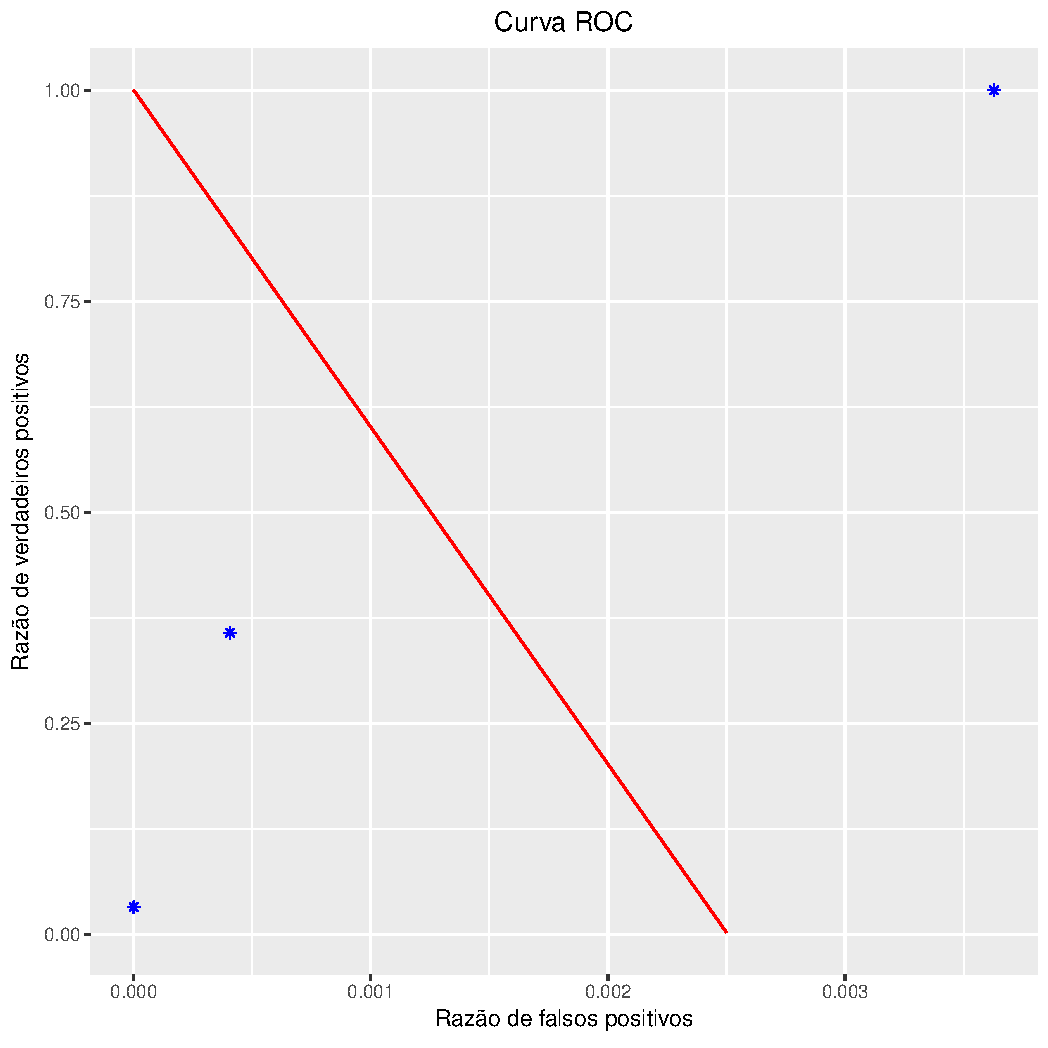
\includegraphics[width=4.0in]{curva_roc_3_canais.pdf}
	\caption{Distribuição diferença de fase {\it n-looks}.}
\label{cap_fusao_fig03}
\end{figure}
%%% ACF O que é a linha vermelha?

Podemos definir a prevalencia
\begin{equation}\label{cap_fusao_25}
	P =\overline{TP_j}+\overline{FN_j}, \\
\end{equation}
e o $Q-$ nível
\begin{equation}\label{cap_fusao_26}
	Q =\overline{TP_j}+\overline{FP_j}, \\
\end{equation}
para cada $j$.


As posições dos pontos nas curvas ROC fornecem informações qualitativas sobre a acurácia da detecção para cada mapa de bordas $M_j$. 

Seja a equação
\begin{equation}\label{cap_fusao_27}
     P^{'}FP_{rate}+P TP_{rate} = Q, \\
\end{equation}
\begin{equation}\label{cap_fusao_28}
     (1-P)\left(1-\frac{TN}{FP+TN}\right)+P \frac{TP}{TP+FN} = Q, \\
\end{equation}
\begin{equation}\label{cap_fusao_29}
     (1-P) \left(\frac{FP+TN-TN}{FP+TN}\right)+TP = Q, \\
\end{equation}
\begin{equation}\label{cap_fusao_30}
     (1-P) \left(\frac{FP}{FP+TN}\right)+TP = Q, \\
\end{equation}
\begin{equation}\label{cap_fusao_31}
      FP\left(\frac{(1-P)}{FP+TN}\right)+TP = Q, \\
\end{equation}

 Lembrando que $TP+FN+FP+TN=1$

\begin{equation}\label{cap_fusao_32}
      FP\left(\frac{FP+TN}{FP+TN}\right)+TP = Q, \\
\end{equation}

\begin{equation}\label{cap_fusao_33}
      FP+TP = Q, \\
\end{equation}

O detector de bordas ótimo tem a propriedade de ser aquele que identifica como borda todos os pixeis de bordas verdadeiros, ou seja, $FP$ e $FN$ deveriam ser zero portanto o detector de borda ideal satisfaz $P=Q$. 


Reescrevendo a equação (\ref{cap_fusao_27}) usando o fato $P=Q$ teremos
\begin{equation}\label{cap_fusao_34}
     P^{'}FP_{rate}+P TP_{rate} = P. \\
\end{equation}

Duas observações podem ser feitas, primeiro, os pontos $(0,1)$ e $(P,P)$ no espaço ROC satisfazem a equação (\ref{cap_fusao_34}). Segundo, usando a mesma equação podemos definir a linha diagnóstico da seguinte maneira
\begin{equation}\label{cap_fusao_35}
     P^{'}FP_{rate}+P TP_{rate} = P, \\
\end{equation}
\begin{equation}\label{cap_fusao_36}
     P TP_{rate} = P - P^{'}FP_{rate}, \\
\end{equation}
\begin{equation}\label{cap_fusao_37}
    TP_{rate} = 1 - \frac{P^{'}}{P}FP_{rate}, \\
\end{equation}
\begin{equation}\label{cap_fusao_38}
    TP_{rate} = 1 - \frac{(1-P)}{P}FP_{rate}, \\
\end{equation}
\begin{equation}\label{cap_fusao_39}
    TP_{rate} = \frac{(P-1)}{P}FP_{rate} + 1. \\
\end{equation}

Analisando a equação (\ref{cap_fusao_39}) podemos constatar que se $FP_{rate}$ tende para zero então $TP_{rate}$ tende para $1$. 

As figuras (\ref{cap_fusao_fig04}), (\ref{cap_fusao_fig05}) e (\ref{cap_fusao_fig06}) mostram as evidências de bordas em cada canal da imagem simulada de duas folhas proposta no capítulo (\ref{cap_acf}), as quais serão usada como imagem de referência para o método de detecção automático. Isto é, mostram $E_1$, $E_2$ e $E_3$.
\begin{figure}[!hbt]
\minipage{0.475\textwidth}
\fbox{  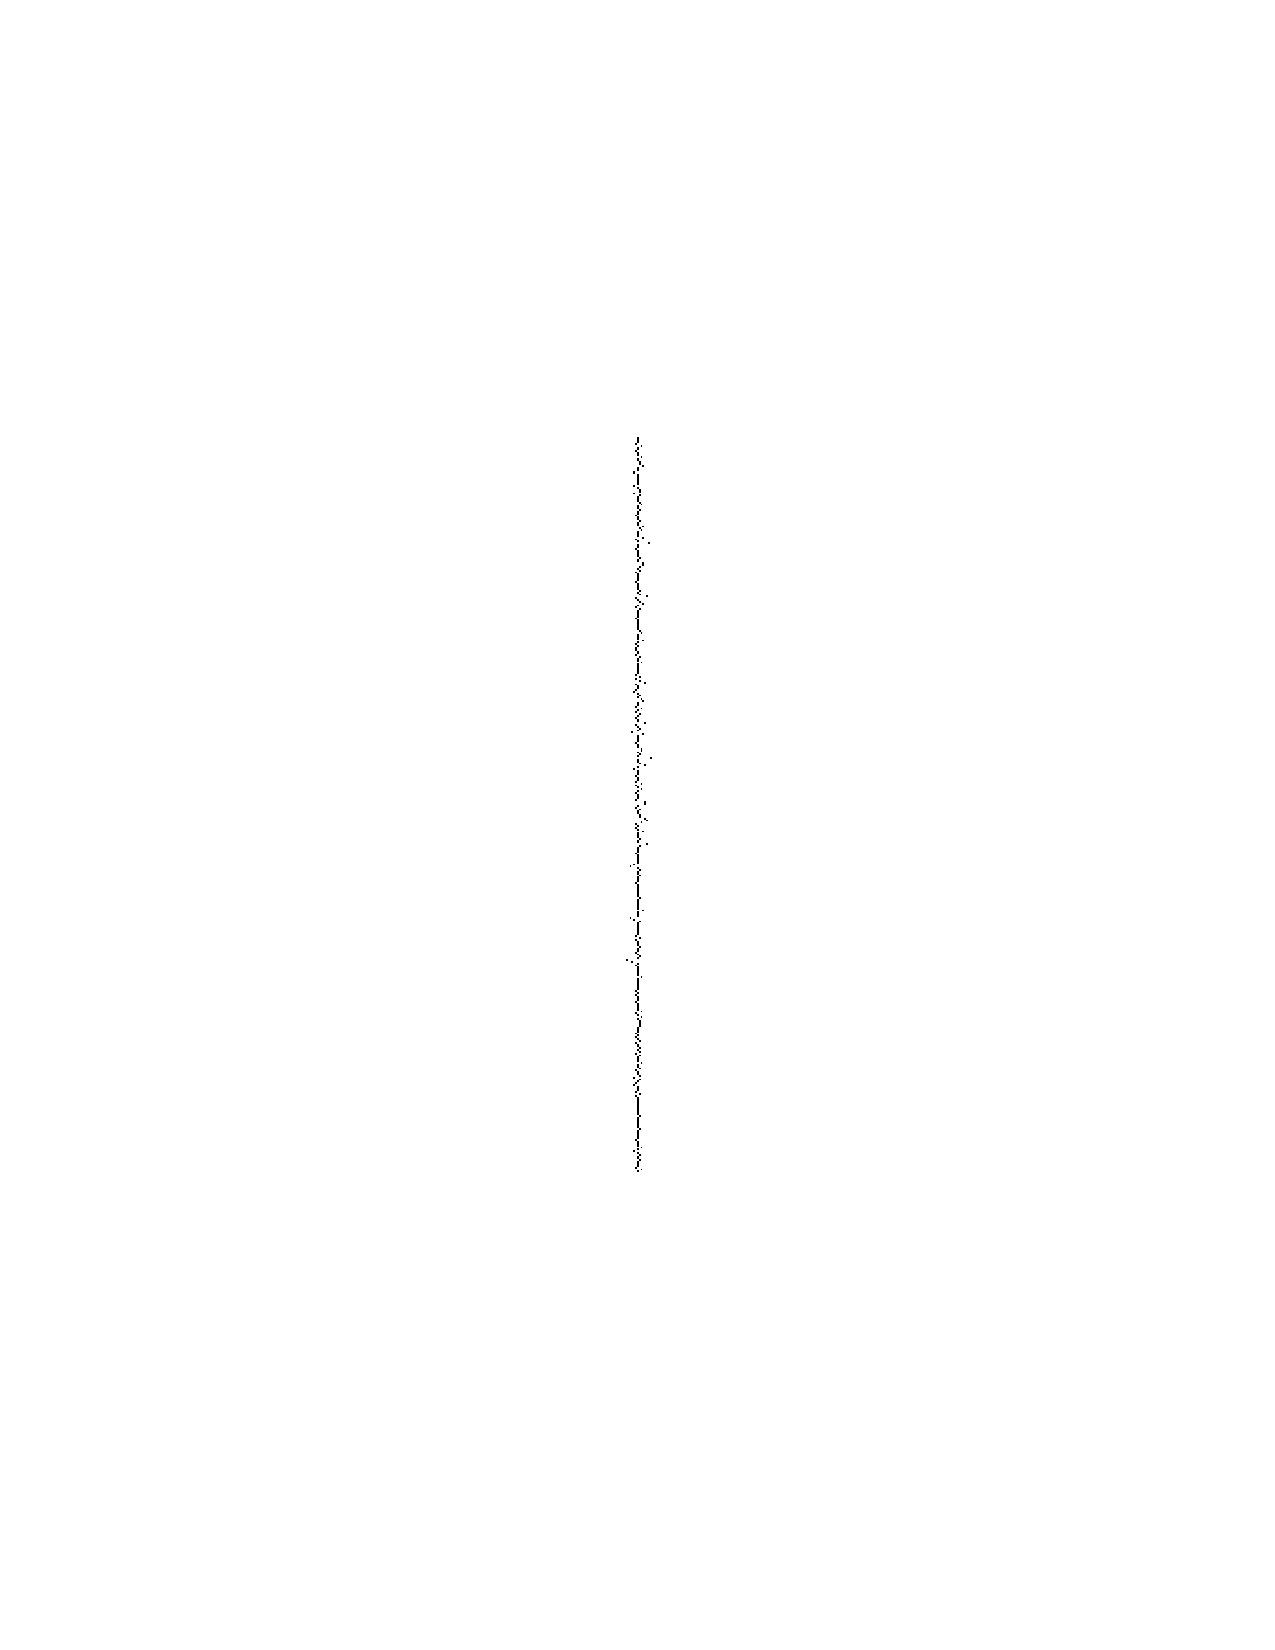
\includegraphics[width=\linewidth]{ev_hh_nhfc_2014.pdf}}
\caption{Evidências de bordas $E_1$ para o canal $I_{HH}$}\label{cap_fusao_fig04}
\endminipage\hfill
\minipage{0.475\textwidth}
\fbox{ 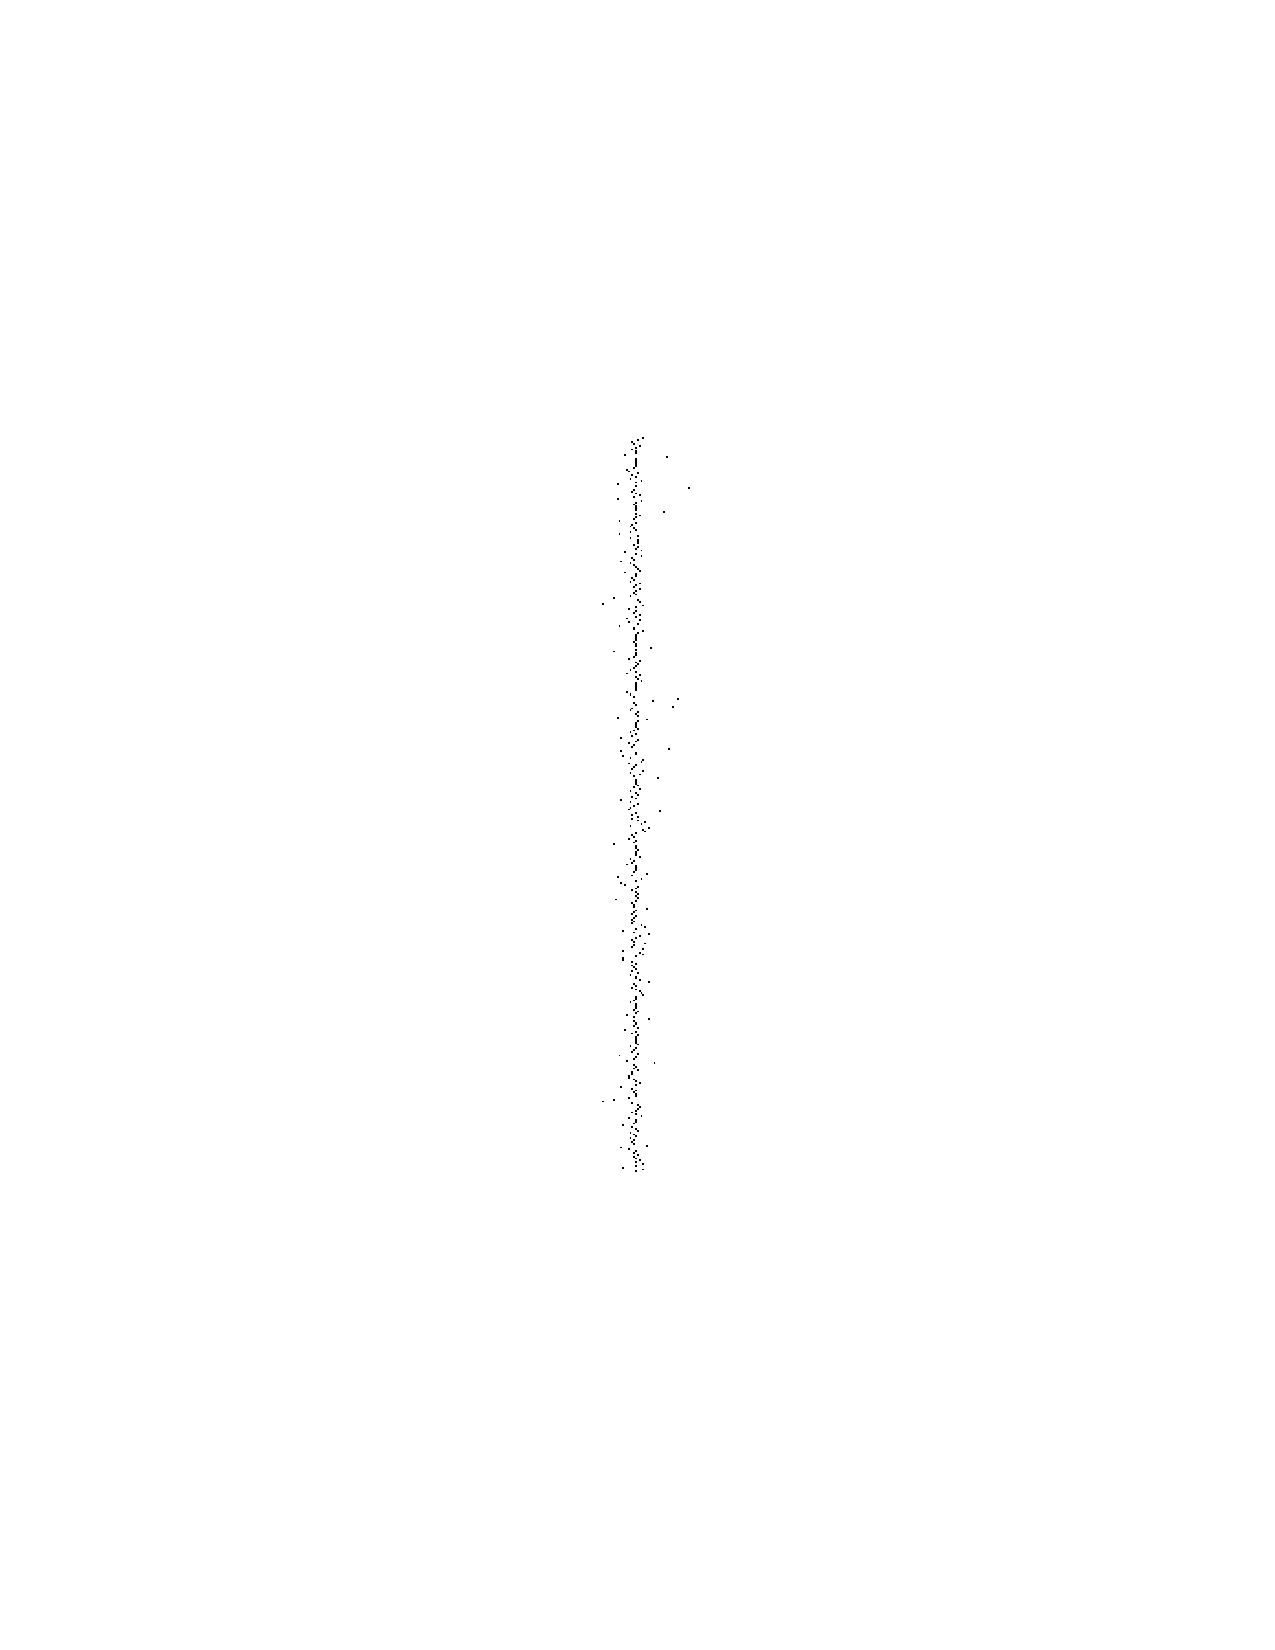
\includegraphics[width=\linewidth]{ev_hv_nhfc_2014.pdf}}
\caption{Evidências de bordas $E_2$ para o canal $I_{HV}$}\label{cap_fusao_fig05}
\endminipage\hfill
\centering
\minipage{0.475\textwidth}
\fbox{ 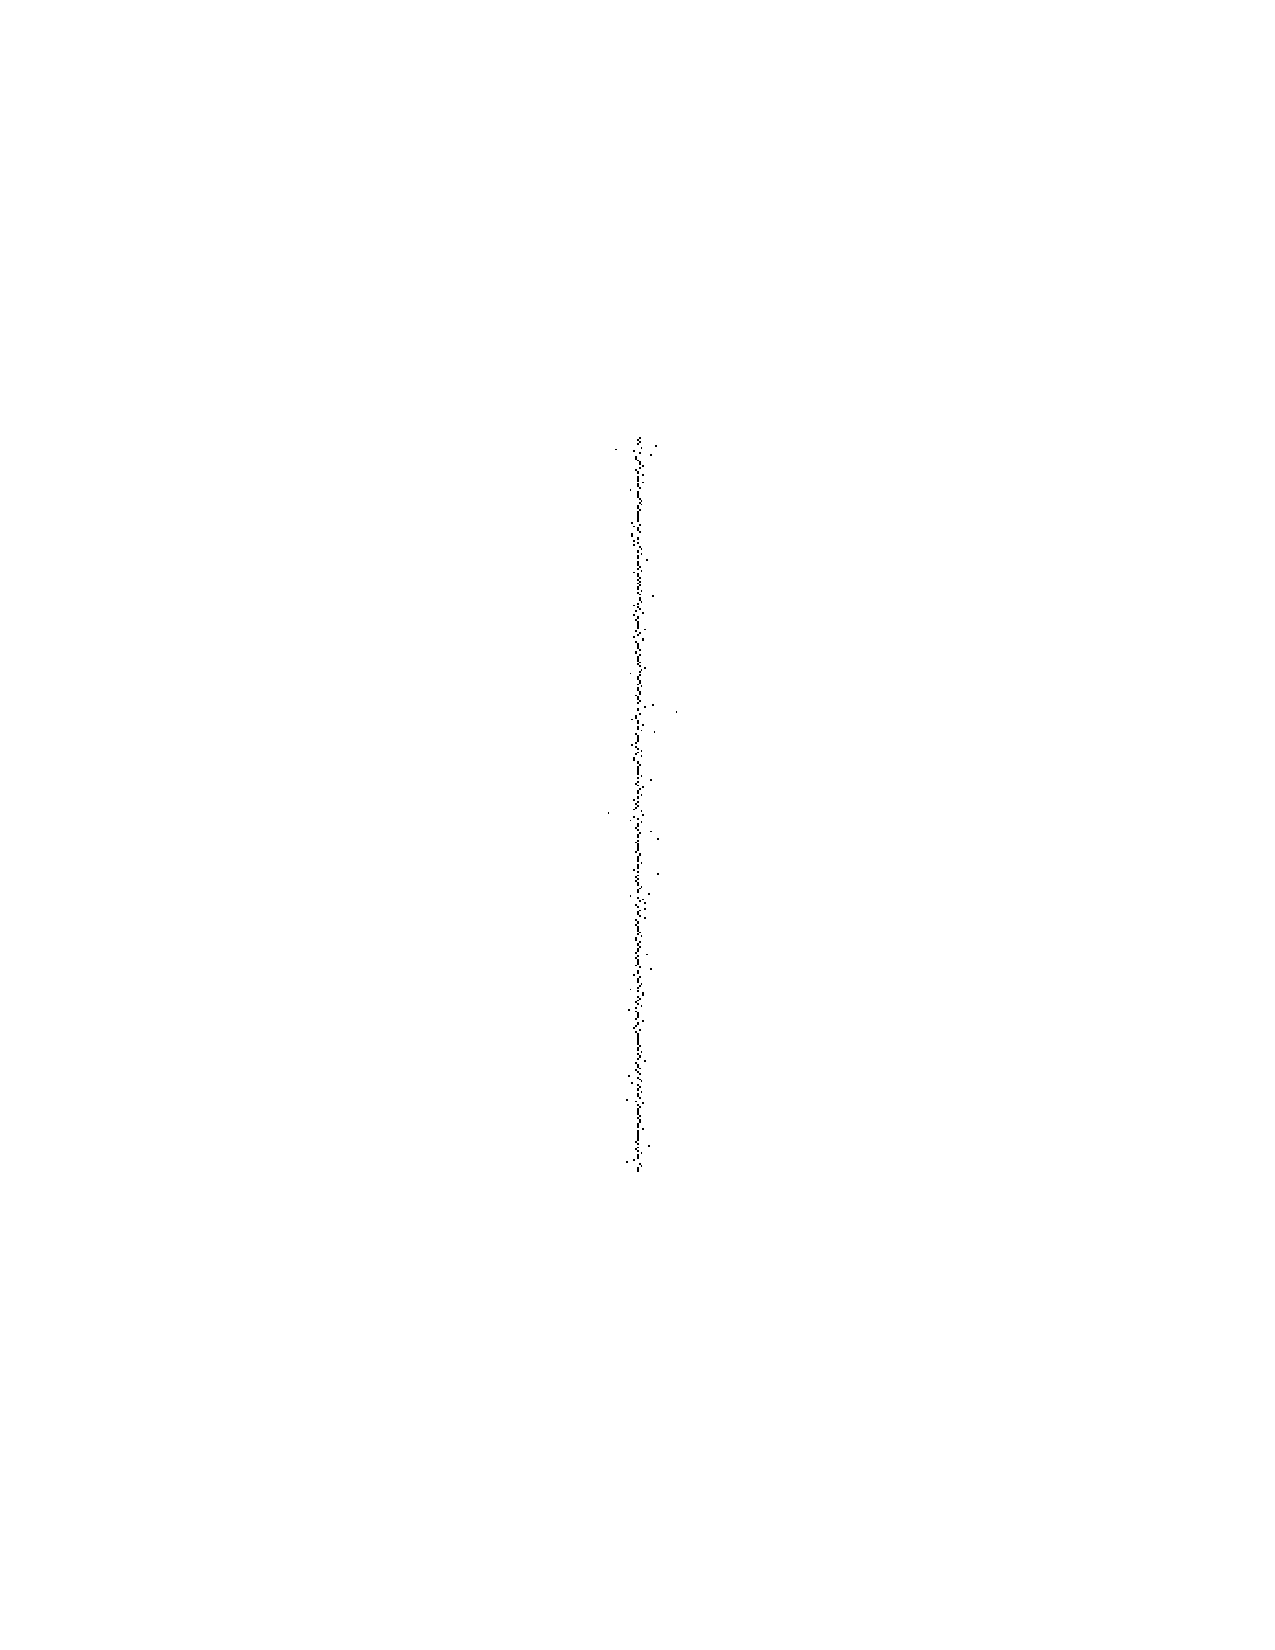
\includegraphics[width=\linewidth]{ev_vv_nhfc_2014.pdf}}
\caption{Evidências de bordas $E_3$ para o canal $I_{VV}$}\label{cap_fusao_fig06}
\endminipage\hfill
\end{figure}


A figura (\ref{cap_fusao_fig07}) mostra a matriz de fusão $F$, com a soma das imagens de referências $E_1$, $E_2$ e $E_3$.

\begin{figure}[!hbt]
\fbox{  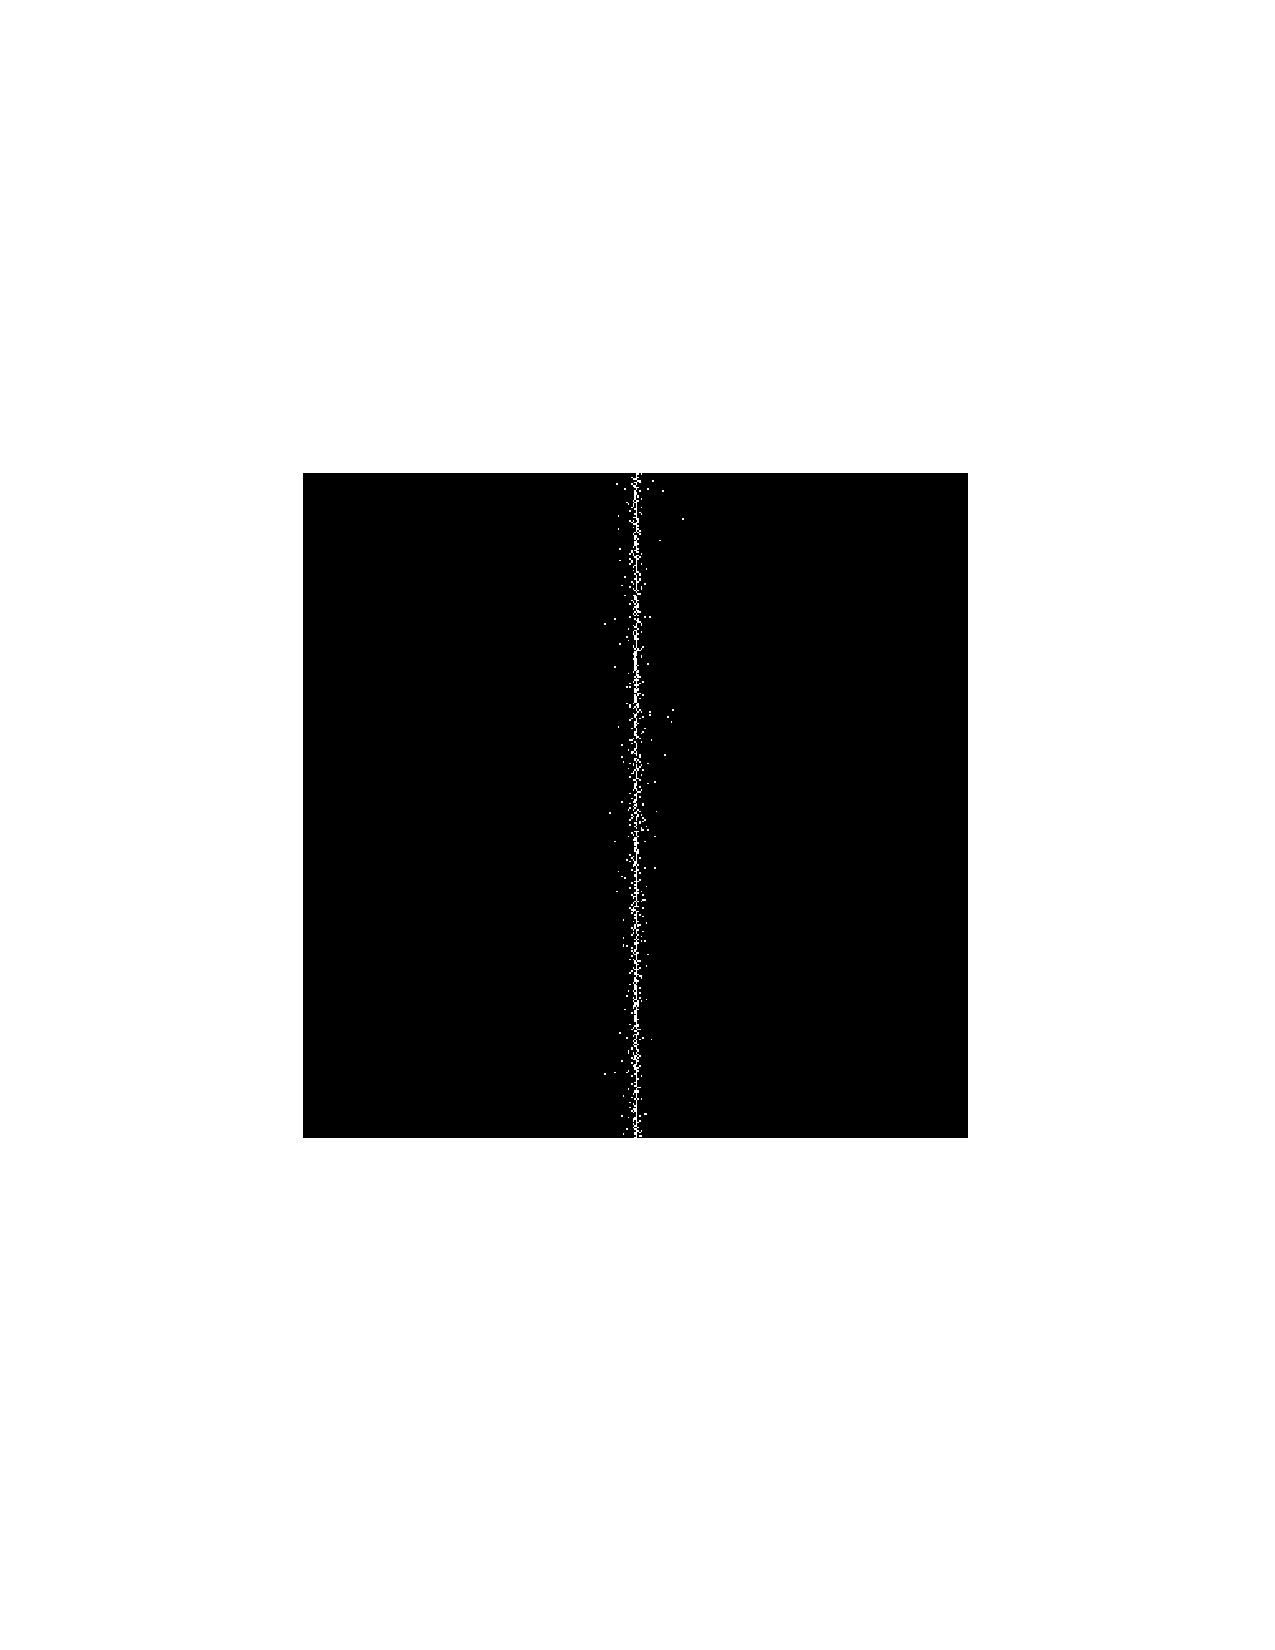
\includegraphics[width=\linewidth]{matriz_soma_v.pdf}}
\caption{Fusão de evidência $F = E_1+E_2+E_3$}\label{cap_fusao_fig07}
\end{figure}

As figuras (\ref{cap_fusao_fig08}), (\ref{cap_fusao_fig09}) e (\ref{cap_fusao_fig10}) mostram os mapas de bordas com limiares. Teremos as imagens $M_1$, $M_2$ e $M_3$ depois de aplicados os respectivos limiares $CT_1$, $CT_2$ e $CT_3$.

\begin{figure}[!hbt]
\minipage{0.475\textwidth}
\fbox{  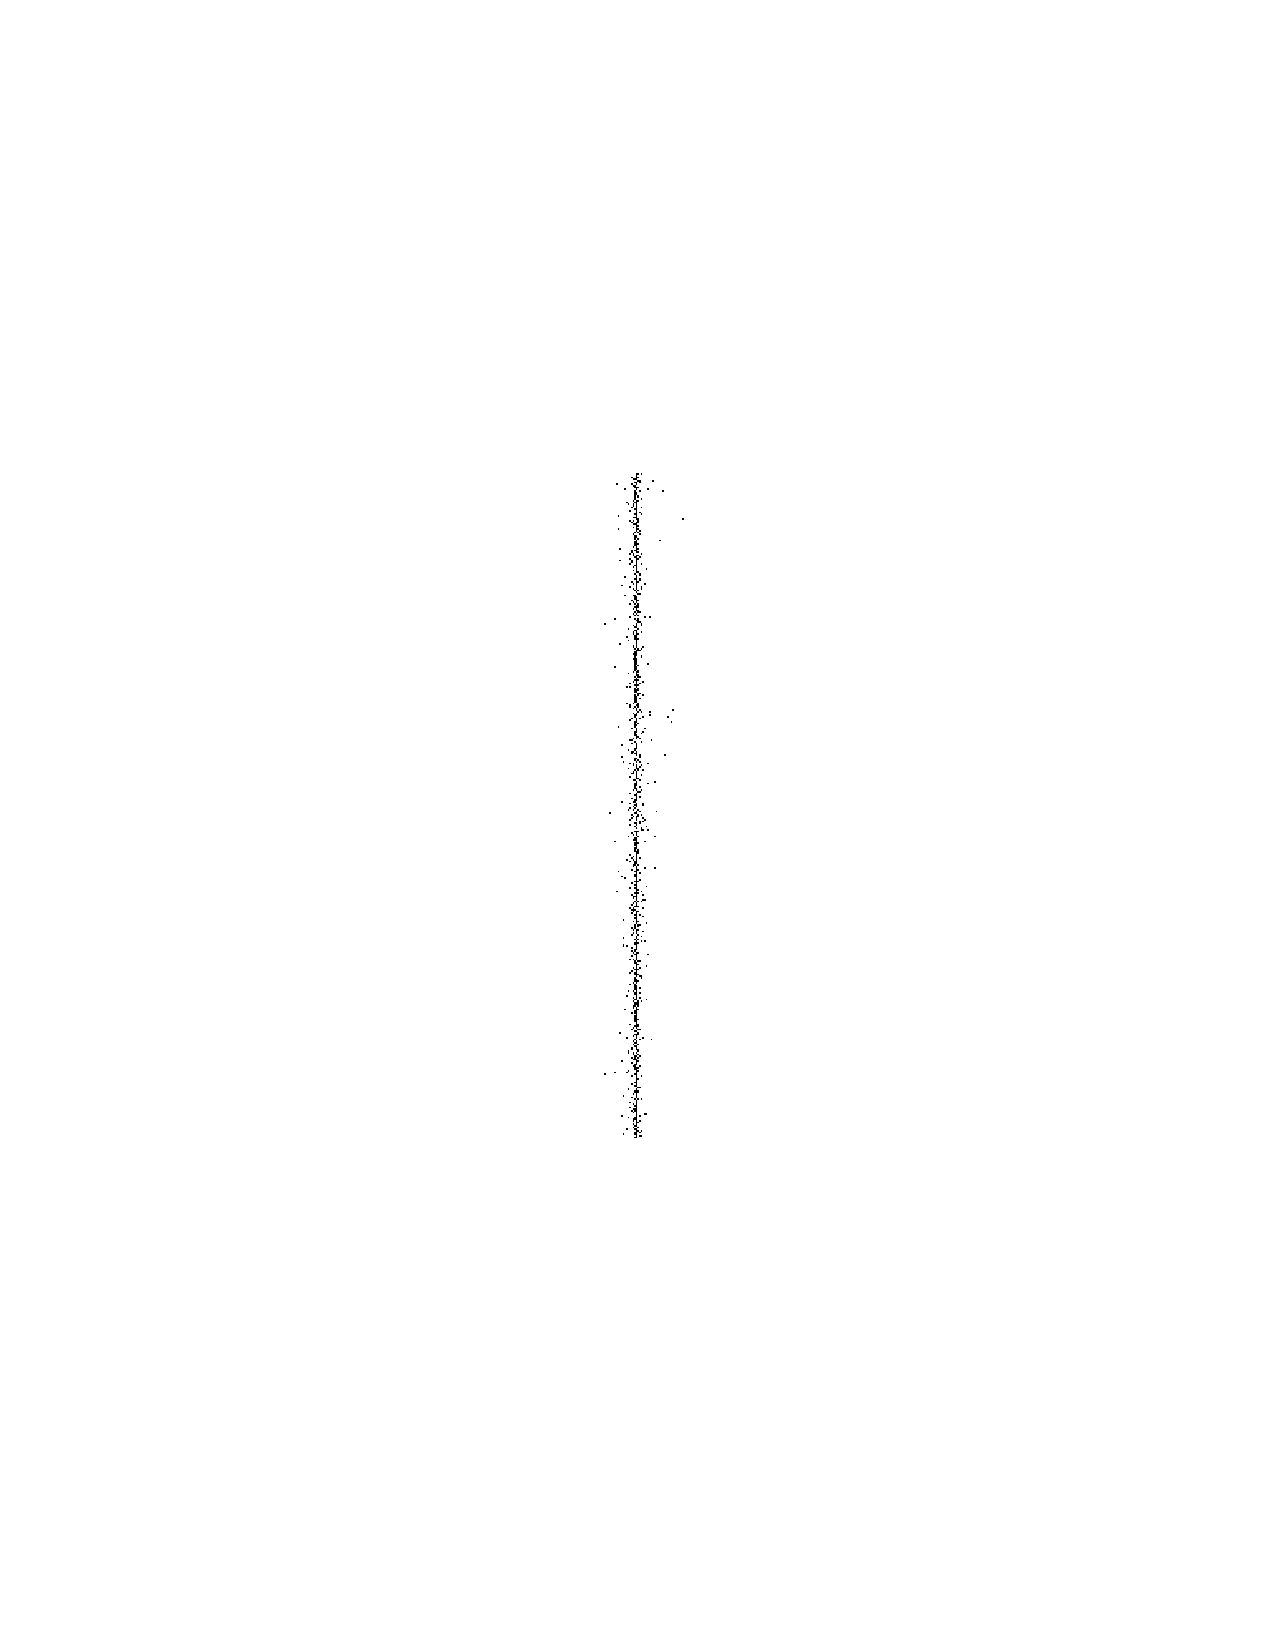
\includegraphics[width=\linewidth]{matriz_limiar_m1_nhfc.pdf}}
\caption{Mapa de borda $M_1$ com limiar $CT_1=1$}\label{cap_fusao_fig08}
\endminipage\hfill
\minipage{0.475\textwidth}
\fbox{ 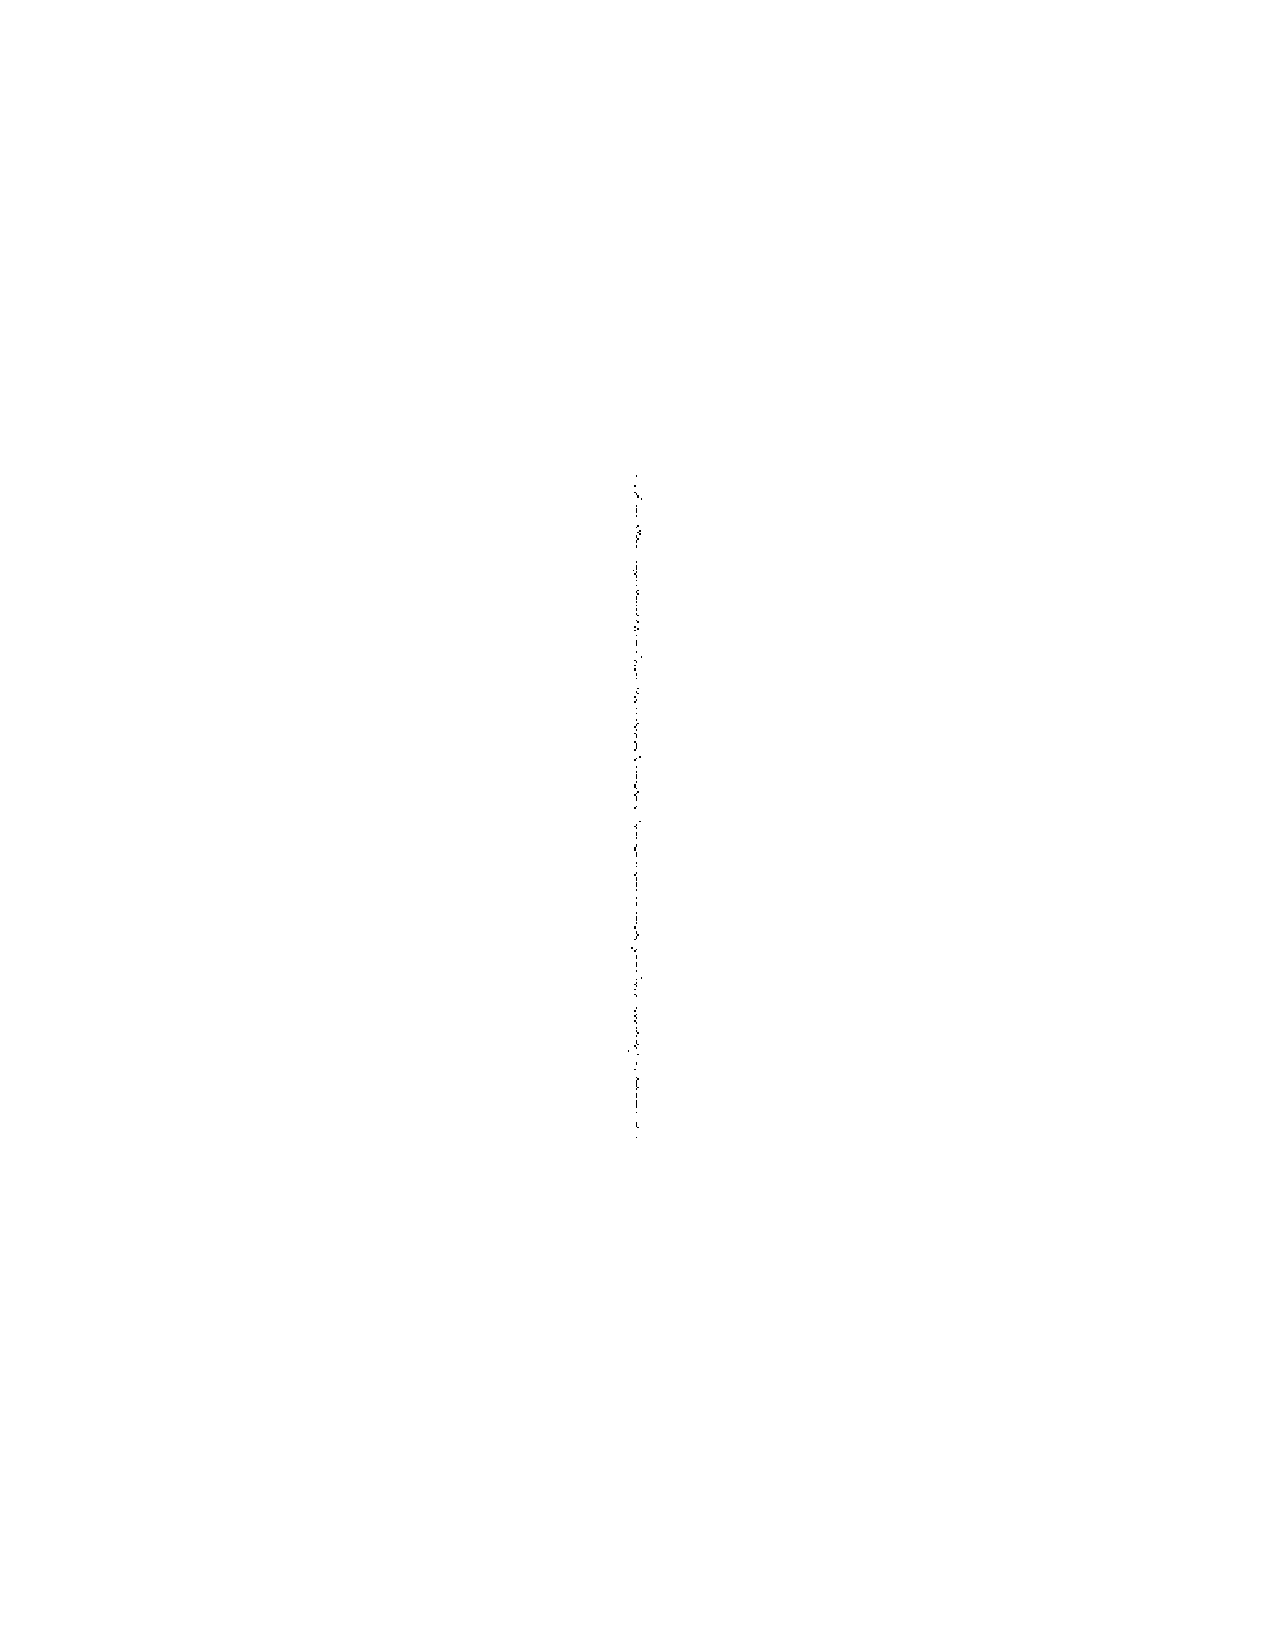
\includegraphics[width=\linewidth]{matriz_limiar_m2_nhfc.pdf}}
\caption{Mapa de borda $M_2$ com limiar $CT_2=2$}\label{cap_fusao_fig09}
\endminipage\hfill
\centering
\minipage{0.475\textwidth}
\fbox{ 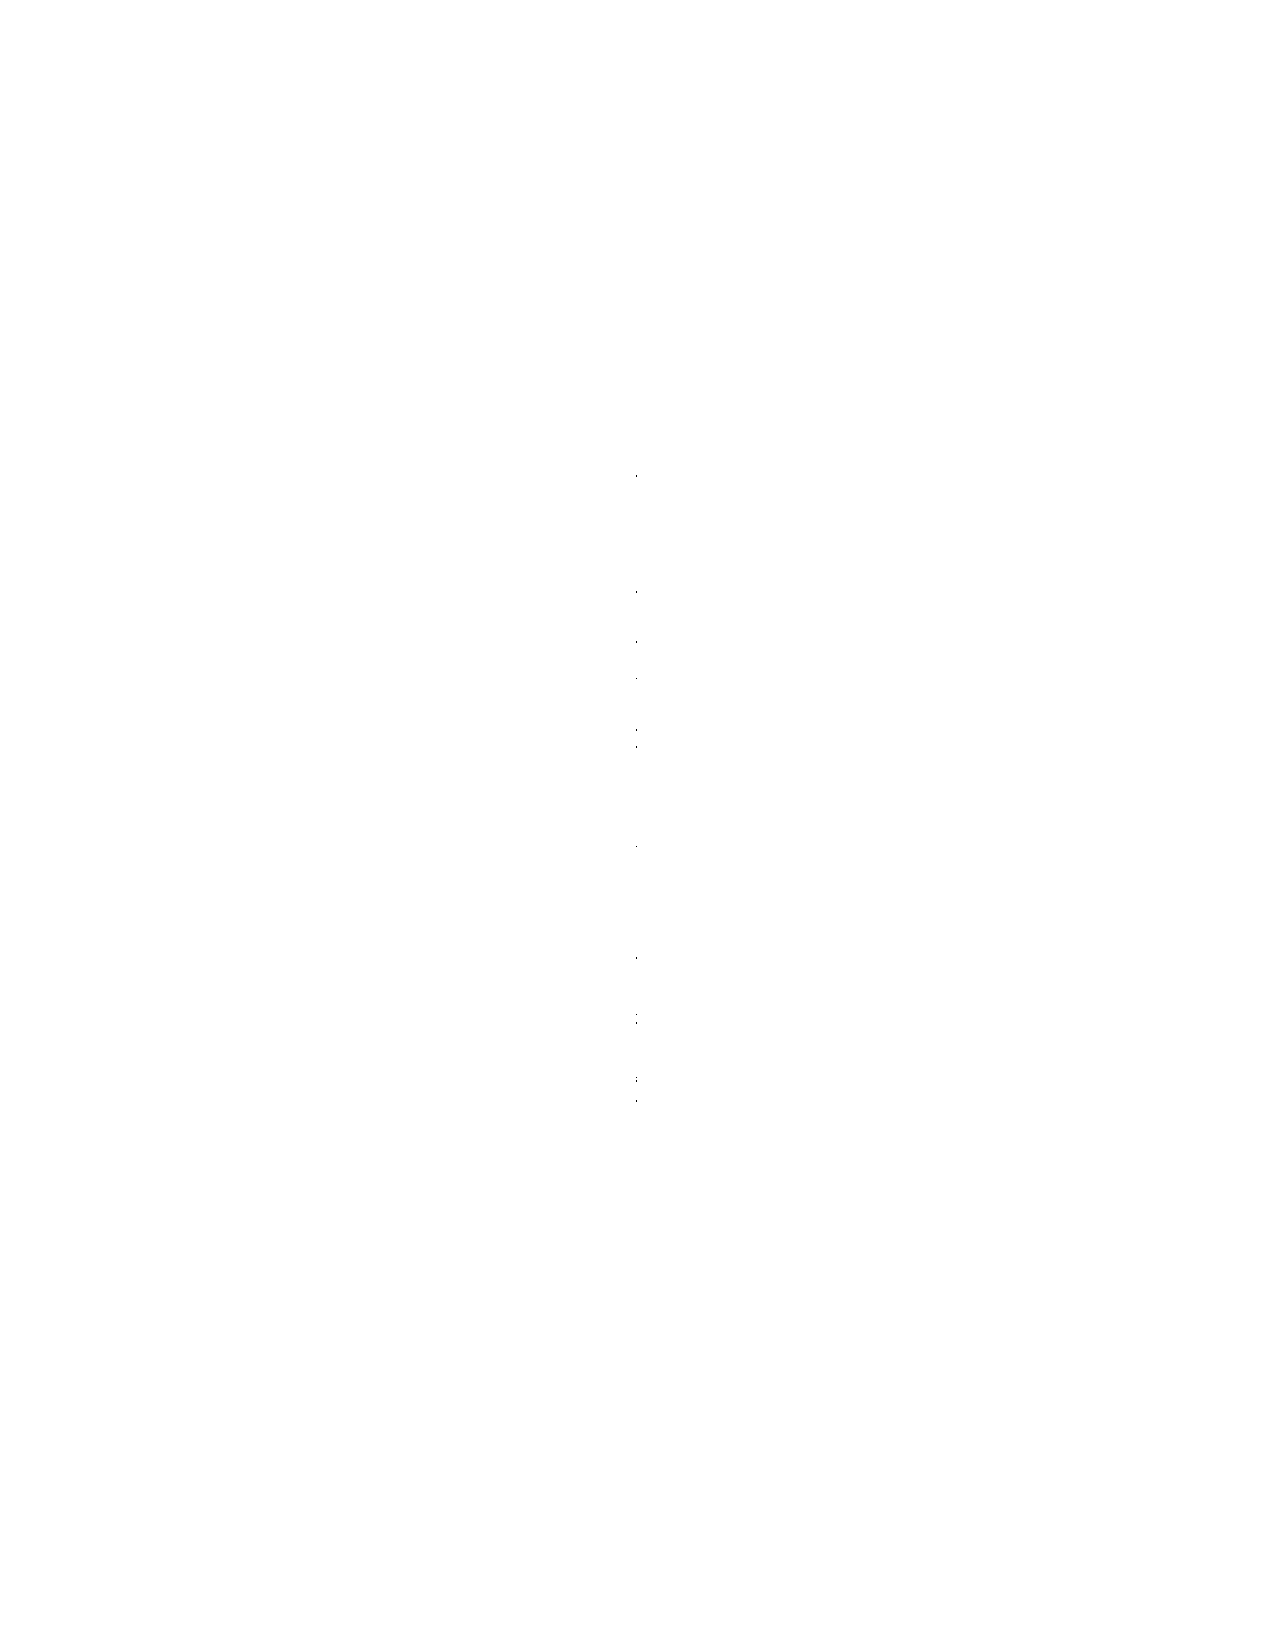
\includegraphics[width=\linewidth]{matriz_limiar_m3_nhfc.pdf}}
\caption{Mapa de borda $M_3$ com limiar $CT_3=3$}\label{cap_fusao_fig10}
\endminipage\hfill
\end{figure}

A curva ROC mostrada na figura (\ref{cap_fusao_fig03}) indica que a melhor escolha para limiar correspondente é $CT=2$, o que podemos comprovar na imagem nas imagens acima.  
\subsection{Coeficientes ponderados $\kappa$ (CP-$\kappa$)}
O coeficiente $\kappa$ descrito nesta seção busca escolher um estimativa para o limiar correspondente resultando em uma fusão de bordas de evidências de bordas acurada.

Definindo o $\kappa$ índice
$$\kappa = \frac{A_0 - A_c}{A_a - A_c},$$
onde $A_0$ é a medida de concordância entre resultados de dois algoritmos de detecção de bordas, $A_c$ é o valor esperado com base na concordância por acaso dos dois detectores de bordas e $A_a$ é o valor esperado com base na concordância completa dos dois detectores de borda, isto é, $A_0=\max\{A_0\}$.

A generalização do coeficiente $\kappa$ pode ser assumindo pesos $w_{u,v}$ $u=1,2$ e $v=1,2$ os quais são atribuídos para os quatro possíveis valores resultados dos processos de detecções de bordas que geram a matriz de confusão. Os pesos caracterizam-se por $0<|w_{u,v}|\le 1$. 

Definindo respectivamente a proporção ponderada observada de concordância entre dois detectores de bordas por 
\begin{equation}\label{cap_fusao_40}
	D_{0_w} =\sum_{u=1}^{2}\sum_{v=1}^{2} w_{u,v}d_{u,v},  \\
\end{equation}
onde $d_{u,v}$ assumem valores da matriz de confusão e são calculado como mostra a tabela (\ref{cap_fusao_tab05}), desenvolvendo a equação teremos,
\begin{equation}\label{cap_fusao_41}
	D_{0_w} =\sum_{u=1}^{2}\sum_{v=1}^{2} w_{u,v}d_{u,v}= w_{1,1}d_{1,1}+w_{1,2}d_{1,2}+w_{2,1}d_{2,1}+w_{2,2}d_{2,2},  \\
\end{equation}
e similarmente é definido a proporção ponderada de acaso esperada de concordância,
\begin{equation}\label{cap_fusao_42}
	D_{C_w} =\sum_{u=1}^{2}\sum_{v=1}^{2} w_{u,v}c_{u,v},  \\
\end{equation}
onde os $c_{u,v}$ referem-se as quatro probabilidades acima, porém no caso detecções de bordas randômicas, isto é, as borda são identificadas puramente por acaso. Podemos ver os valores na tabela (\ref{cap_fusao_05}), desenvolvendo a equação teremos,  
\begin{equation}\label{cap_fusao_43}
	D_{C_w} =\sum_{u=1}^{2}\sum_{v=1}^{2} w_{u,v}d_{u,v}= w_{1,1}c_{1,1}+w_{1,2}c_{1,2}+w_{2,1}c_{2,1}+w_{2,2}c_{2,2}.  \\
\end{equation}

As probabilidades são descritas  conforme a tabela~\ref{cap_fusao_tab04},
em que o índice sobrescrito representa o complemento da grandeza representada.
 
\begin{table}[hbt]
	\centering
	\caption{Probabilidade para as bordas detectadas e as encontradas randômicamente.}\label{cap_fusao_tab04}
\begin{tabular}{@{}lll@{}} \toprule
	     & Bordas detectadas  & Bordas randômicas  \\ \midrule
	TP  & $d_{1,1}=P    \cdot SE$     & $c_{1,1}=P    \cdot Q$  \\ 
	FP  & $d_{1,2}=P^{'}\cdot SP^{'}$ & $c_{1,2}=P^{'}\cdot Q$  \\ 
	FN  & $d_{2,1}=P    \cdot SE^{'}$ & $c_{2,1}=P    \cdot Q^{'}$  \\ 
	TN  & $d_{2,2}=P^{'}\cdot SP$     & $c_{2,2}=P^{'}\cdot Q^{'}$  \\ \bottomrule 
\end{tabular}
\end{table}


Verificando as definições de $d_{u,v}$,
\begin{equation}\label{cap_fusao_44}
	d_{1,1}=P\cdot SE = (TP + FN)\frac{TP}{TP + FN}=TP,
\end{equation}
então $d_{1,1}= TP$.

Para a verificação de $d_{1,2}$ lembrar que $TP+FP+FN+TN=1$ ou $TN+FP=1-TP-FN$, 
\begin{equation}\nonumber
	d_{1,2}=P^{'}\cdot SP^{'} = P^{'}(1-SP)=P^{'} \left(1-\frac{TN}{TN+FP}\right),
\end{equation}
\begin{equation}\nonumber
	d_{1,2}=P^{'}\left(\frac{FP}{TN+FP}\right)=(1-P)\left(\frac{FP}{TN+FP}\right),
\end{equation}
\begin{equation}\nonumber
	d_{1,2}=\left(\frac{FP}{TN+FP}\right)-P\left(\frac{FP}{TN+FP}\right),
\end{equation}
\begin{equation}\nonumber
	d_{1,2}=FP\left[\left(\frac{1}{TN+FP}\right)-P\left(\frac{1}{TN+FP}\right)\right],
\end{equation}
\begin{equation}\nonumber
	d_{1,2}=FP\left[\left(\frac{1 - P}{TN+FP}\right)\right]=FP\left[\left(\frac{1 - TP - FN}{TN+FP}\right)\right],
\end{equation}
 
\begin{equation}\label{cap_fusao_45}
	d_{1,2}=FP=FP\left[\left(\frac{TN+FP}{TN+FP}\right)\right] = FP,
\end{equation}
então $d_{1,2}= FP$.

Sendo agora $d_{2,1}$
\begin{equation}\nonumber
	d_{2,1}=P\cdot SE^{'} = P(1-SE)=P-PSE=P-P\frac{TP}{TP + FN},
\end{equation}
\begin{equation}\nonumber
	d_{2,1}=TP+FN-(TP + FN)\frac{TP}{TP + FN},
\end{equation}
\begin{equation}\label{cap_fusao_46}
	d_{2,1}=TP+FN-TP=FN,
\end{equation}
assim $d_{2,1} = FN$.

Sendo agora $d_{2,2}$
\begin{equation}\nonumber
	d_{2,2}=P^{'}\cdot SP = (1-P)\left(\frac{TN}{TN + FP}\right),
\end{equation}
\begin{equation}\nonumber
	d_{2,2}=\frac{TN}{TN + FP}-\frac{PTN}{TN + FP}=TN\left(\frac{1-P}{TN + FP}\right),
\end{equation}
\begin{equation}\label{cap_fusao_47}
	d_{2,2}=TN\left(\frac{1-TP-FN}{TN + FP}\right)=TN\left(\frac{TN+FP}{TN + FP}\right)=TN,
\end{equation}
então $d_{2,2}=TN$.


E para finalizar é verificado a probabilidade de bordas randômicas.
\begin{equation}\nonumber
	P\cdot Q + P^{'}\cdot Q+P\cdot Q^{'} + P^{'}\cdot Q^{'} = 1.
\end{equation}
\begin{equation}\nonumber
	(P + P^{'})\cdot Q + (P + P^{'}) \cdot Q^{'} = 1.
\end{equation}
\begin{equation}\nonumber
	(P + 1 -P)\cdot Q + (P + 1 - P) \cdot Q^{'} = 1.
\end{equation}
\begin{equation}\nonumber
	 Q +  Q^{'} = 1.
\end{equation}
\begin{equation}\nonumber
	 Q + (1 - Q) = 1.
\end{equation}
Ocorrendo assim a verificação,
\begin{equation}\nonumber
	 1 = 1.
\end{equation}


Baseado na definição do índice $\kappa$ definimos o índice $\kappa$ ponderado como,
\begin{equation}\label{cap_fusao_48}
\kappa_w = \frac{D_{0_w} - D_{C_w}}{\max(D_{0_w} - D_{C_w})}.
\end{equation}

 Usando as definições de $D_{0_w}$ e $D_{C_w}$ mostrada respectivamente na equações (\ref{cap_fusao_40}) e (\ref{cap_fusao_42}) e realizando algumas manipulações algébricas, 
\begin{equation}\nonumber
	D_{0_w} - D_{C_w}=\sum_{u=1}^{2}\sum_{v=1}^{2}w_{u,v}(d_{u,v}- c_{u,v}).
\end{equation}
\begin{equation}\nonumber
	D_{0_w} - D_{C_w}=\sum_{u=1}^{2}\left[w_{u,1}(d_{u,1}- c_{u,1}) + w_{u,1}(d_{u,2}- c_{u,2}) \right].
\end{equation}
\begin{equation}\label{cap_fusao_49}
	D_{0_w} - D_{C_w}=w_{1,1}(d_{1,1}- c_{1,1}) + w_{2,1}(d_{2,2}- c_{2,2}) + w_{1,2}(d_{1,2}- c_{1,2}) + w_{2,2}(d_{2,2}- c_{2,2}).
\end{equation}

De acordo com as definições na matriz de confusão mostradas na tabela (\ref{cap_fusao_tab05}) podemos rescrever a equação (\ref{cap_fusao_49}), 
\begin{equation}\nonumber
	D_{0_w} - D_{C_w}=w_{1,1}(P\cdot SE- P\cdot Q) + w_{2,1}(P^{'}\cdot SP^{'}- P^{'}\cdot Q) + w_{1,2}(P\cdot SE^{'}- P\cdot Q^{'}) + w_{2,2}(P^{'}\cdot SP- P^{'}\cdot Q^{'}).
\end{equation}

Definindo os índices de sensibilidade e de especificidade respectivamente por
\begin{equation}\label{cap_fusao_50}
	\kappa(1,0) = \frac{SE-Q}{Q^{'}}
\end{equation}
\begin{equation}\label{cap_fusao_51}
	\kappa(0,0) = \frac{SP-Q^{'}}{Q}
\end{equation}

\begin{equation}\nonumber
	D_{0_w} - D_{C_w}=w_{1,1}PQ^{'}(\frac{SE-Q}{Q^{'}}) + w_{2,1}P^{'}(SP^{'}- Q) + w_{1,2}P(SE^{'}-Q^{'}) + w_{2,2}P^{'}(\frac{SP-Q^{'}}{Q}).
\end{equation}
\begin{equation}\label{cap_fusao_52}
	D_{0_w} - D_{C_w}=w_{1,1}PQ^{'}\kappa(1,0) + w_{2,1}P^{'}(SP^{'}- Q) + w_{1,2}P(SE^{'}-Q^{'}) + w_{2,2}P^{'}\kappa(0,0).
\end{equation}

O coeficiente de ponderação pode representar ganho ou perda da propriedade que acompanha e podemos afirmar que varia entre $0$ e $1$, dependendo da acurácia do detector de bordas, portanto, $0\le w_{u,v}\le 1$, com $u=1,2$ e $v=1,2$.

Observando a equação $\ref{cap_fusao_52}$ podemos supor que o custo total para as bordas verdadeira serem propriamente identificadas como bordas ou não é igual a 
\begin{equation}\label{cap_fusao_53}
	W_1= |w_{1,1}| +|w_{2,1}|,
\end{equation}
da mesma forma, $W_2$ é o custo total para um pixel de não borda e definido como
\begin{equation}\label{cap_fusao_54}
	W_2= |w_{1,2}| +|w_{2,1}|.
\end{equation}

Sem perda de generalidade custo total pode ser dividido uniformemente, isto é, $w_{1,1}= \frac{W_1}{2}$ e $w_{2,1}=-\frac{W_1}{2}$, e ainda $w_{1,2}=-\frac{W_2}{2}$ e $w_{2,2}=\frac{W_2}{2}$, desta maneira a equação (\ref{cap_fusao_52}) pode ser reescrita
\begin{equation}\label{cap_fusao_55}
	D_{0_w} - D_{C_w}=\frac{W_1}{2}PQ^{'}\kappa(1,0) - \frac{W_2}{2}P^{'}(SP^{'}- Q) - \frac{W_1}{2}P(SE^{'}-Q^{'}) + \frac{W_2}{2}P^{'}Q\kappa(0,0),
\end{equation}
lembrando que $P=1-P^{'}$, $Q=1-Q^{'}$, $SP=1-SP^{'}$ e $SE=1-SE^{'}$
\begin{equation}\label{cap_fusao_56}
	D_{0_w} - D_{C_w}=\frac{W_1}{2}P\left(Q^{'}\kappa(1,0) - SE^{'}+Q^{'}\right) +\frac{W_2}{2}P^{'}\left(Q\kappa(0,0)-SP^{'}+Q\right).
\end{equation}

Considerando cada um dos termos da soma separadamente, teremos
\begin{equation}\nonumber
	\begin{array}{lll}
		Q^{'}\kappa(1,0) - SE^{'}+Q^{'}&=& Q^{'}\left(\frac{SE-Q}{2}\right) - SE^{'}+ 1 - Q \\
		Q^{'}\kappa(1,0) - SE^{'}+Q^{'}&=& (SE-Q) - (SE- 1) + 1 - Q.\\
		Q^{'}\kappa(1,0) - SE^{'}+Q^{'}&=& 2(SE-Q).\\
	\end{array}	
\end{equation}
\begin{equation}\nonumber
	\begin{array}{lll}
		\left(Q\kappa(0,0)-SP^{'}+Q\right)&=&Q\left(\frac{SP-Q^{'}}{Q}-SP^{'}+Q\right)\\
		\left(Q\kappa(0,0)-SP^{'}+Q\right)&=&SP-Q^{'}+SP+1-Q^{'}-1\\
		\left(Q\kappa(0,0)-SP^{'}+Q\right)&=&2(SP-Q^{'})\\
	\end{array}	
\end{equation}
portanto, a equação (\ref{cap_fusao_56})
\begin{equation}\label{cap_fusao_57}
	\begin{array}{lll}
		D_{0_w} - D_{C_w}&=&W_1P(SE-Q) +W_2P^{'}(SP - Q^{'})\\
		D_{0_w} - D_{C_w}&=&W_1PQ^{'}\frac{(SE-Q)}{Q^{'}} +W_2P^{'}Q\frac{(SP - Q^{'})}{Q}\\
		D_{0_w} - D_{C_w}&=&W_1PQ^{'}\kappa(1,0) +W_2P^{'}Q\kappa(0,0)\\
	\end{array}	
\end{equation}

O denominador na equação (\ref{cap_fusao_57}) é definido como 
\begin{equation}\nonumber
	\begin{array}{lll}
		\max(D_{0_w} - D_{C_w})&=&\max(W_1PQ^{'}\kappa(1,0) +W_2P^{'}Q\kappa(0,0)),\\
	\end{array}	
\end{equation}
os coeficientes $\kappa(1,0)$ e $\kappa(0,0)$ alcançam seu valor máximo em $1$, 
\begin{equation}\label{cap_fusao_58}
	\begin{array}{lll}
		\max(D_{0_w} - D_{C_w})&=&W_1PQ^{'} +W_2P^{'}Q.\\
	\end{array}	
\end{equation}

Usando o numerador e denominador deduzidos e substituindo as equações (\ref{cap_fusao_57}) e (\ref{cap_fusao_58}) na equação (\ref{cap_fusao_56}) teremos  

\begin{equation}\label{cap_fusao_59}
\kappa_w = \frac{W_1PQ^{'}\kappa(1,0) +W_2P^{'}Q\kappa(0,0)}{W_1PQ^{'} +W_2P^{'}Q}.
\end{equation}

Continuando com as operações algébricas podemos dividir o numerado e o denominador por $W_1 + W_2$
\begin{equation}\label{cap_fusao_60}
	\kappa_w = \frac{\frac{W_1}{W_1+W_2}PQ^{'}\kappa(1,0) +\frac{W_2}{W_1+W_2}P^{'}Q\kappa(0,0)}{\frac{W_1}{W_1+W_2}PQ^{'} +\frac{W_2}{W_1+W_2}P^{'}Q}.
\end{equation}

Definindo $r=\frac{W_1}{W_1+W_2}$ e $r^{'}=1-r$, teremos
\begin{equation}\nonumber
	\begin{array}{lll}
		r^{'}&=&1-r\\
		r^{'}&=&1-\frac{W_1}{W_1+W_2}\\
		r^{'}&=&\frac{W_1+W_2-W_1}{W_1+W_2}\\
		r^{'}&=&\frac{W_2}{W_1+W_2},\\
	\end{array}	
\end{equation}
portanto a equação (\ref{cap_fusao_60}) pode ser reescrita como
\begin{equation}\label{cap_fusao_61}
	\kappa_r = \frac{rPQ^{'}\kappa(1,0) +r^{'}P^{'}Q\kappa(0,0)}{rPQ^{'} +r^{'}P^{'}Q}.
\end{equation}

Para um valor selecionado $r$ o coeficiente $\kappa_r$ ponderado $\kappa_j(r,0)$ é calculado para cada mapa de borda como na equação (\ref{cap_fusao_61}). O limiar ótimo $CT$ é escolhido de forma a maximizar o coeficientes $\kappa$ ponderados e indica a qualidade da detecção de bordas. 


\begin{table}[hbt]
	\centering
	\caption{Coeficientes $\kappa$ para $r=0.5$.}\label{cap_fusao_tab05}
\begin{tabular}{@{}ll@{}} \toprule
	     & $\kappa_j(r,0)$  \\ \midrule
	$j=1$  & $\kappa_1(r,0)= 0.5786$    \\ 
	$j=2$  & $\kappa_2(r,0)= 0.4694$    \\ 
    $j=3$  & $\kappa_3(r,0)= 0.0628$    \\ \bottomrule 
\end{tabular}
\end{table}

\subsection{A ideia geométrica do índice $\kappa$ ponderado}

Partindo da equação (\ref{cap_fusao_61}) e realizando operações algébricas teremos
\begin{equation}\nonumber
	\kappa_r (rPQ^{'} +r^{'}P^{'}Q)= rPQ^{'}\kappa(1,0) +r^{'}P^{'}Q\kappa(0,0).
\end{equation}
\begin{equation}\nonumber
	\kappa_r rPQ^{'} +\kappa_r r^{'}P^{'}Q= rPQ^{'}\kappa(1,0) +r^{'}P^{'}Q\kappa(0,0).
\end{equation}
\begin{equation}\nonumber
	\kappa_r rPQ^{'}-rPQ^{'}\kappa(1,0) = -( \kappa_r r^{'}P^{'}Q-r^{'}P^{'}Q\kappa(0,0)).
\end{equation}
\begin{equation}\nonumber
	rPQ^{'}(\kappa_r-\kappa(1,0)) = -r^{'}P^{'}Q( \kappa_r -\kappa(0,0)).
\end{equation}
\begin{equation}\label{cap_fusao_62}
	(\kappa_r-\kappa(1,0)) = - \frac{-r^{'}P^{'}Q}{rPQ^{'}}\left( \kappa_r -\kappa(0,0)\right).
\end{equation}
resultando na equação da reta com inclinação $s$, onde $s$ é calculado como,
\begin{equation}\label{cap_fusao_63}
	s = - \frac{-r^{'}P^{'}Q}{rPQ^{'}}.
\end{equation}
ou 
\begin{equation}\label{cap_fusao_64}
	s = \frac{\kappa_r-\kappa(1,0)}{ \kappa_r -\kappa(0,0)} = - \frac{-r^{'}P^{'}Q}{rPQ^{'}}.
\end{equation}
portanto $s$ é o coeficiente angular de uma reta definida como reta projeção $r$.


\subsection{A derivada do coeficiente $\kappa$ ponderado}
Seja a equação para os coeficientes $\kappa$ ponderado (\ref{cap_fusao_61})
\begin{equation}\nonumber
	\kappa_r = \frac{rPQ^{'}\kappa(1,0) +r^{'}P^{'}Q\kappa(0,0)}{rPQ^{'} +r^{'}P^{'}Q}.
\end{equation}
Relembrando os índices de sensibilidade e de especificidade respectivamente
\begin{equation}\nonumber
	\kappa(1,0) = \frac{SE-Q}{Q^{'}},
\end{equation}
\begin{equation}\nonumber
	\kappa(0,0) = \frac{SP-Q^{'}}{Q}
\end{equation}
Podemos escrever 
\begin{equation}\nonumber
	\kappa_r = \frac{rPQ^{'}\frac{SE-Q}{Q^{'}} +r^{'}P^{'}Q\frac{SP-Q^{'}}{Q}}{rPQ^{'} +r^{'}P^{'}Q},
\end{equation}
implicando em,
\begin{equation}\label{cap_fusao_65}
	\kappa_r = \frac{rP(SE-Q) + r^{'}P^{'}(SP-Q^{'})}{rPQ^{'} +r^{'}P^{'}Q}.
\end{equation}

A tabela (\ref{cap_fusao_06}) mostra a matriz de confusão redefinida para a definição de desvio padrão. 
\begin{table}[hbt]
	\centering
	\caption{Matriz de confusão com desvio padrão.}\label{cap_fusao_tab06}
\begin{tabular}{@{}ccc@{}} \toprule
	     & Bordas detectadas  & Bordas randômicas  \\ \midrule
	TP  & $P\cdot Q +\rho \sigma_p\sigma_q=P\cdot SE$         & $P\cdot Q$  \\ 
	FP  & $P^{'}\cdot Q -\rho \sigma_p\sigma_q=P^{'}\cdot SP^{'}$ & $P^{'}\cdot Q$  \\ 
	FN  & $P\cdot Q^{'} -\rho \sigma_p\sigma_q=P    \cdot SE^{'}$ & $P    \cdot Q^{'}$  \\ 
	TN  & $P^{'}\cdot Q^{'} +\rho \sigma_p\sigma_q=P^{'}\cdot SP$     & $P^{'}\cdot Q^{'}$  \\ \bottomrule 
\end{tabular}
\end{table}

Portanto
\begin{equation}\nonumber
	P(SE-Q) = \rho \sigma_p\sigma_q,
\end{equation}
e 
\begin{equation}\nonumber
	P^{'}(SP-Q^{'}) = \rho \sigma_p\sigma_q.
\end{equation}

Substituindo na equação (\ref{cap_fusao_65}), teremos
\begin{equation}\nonumber
	\kappa_r = \frac{r\rho \sigma_p\sigma_q + r^{'}\rho \sigma_p\sigma_q}{rPQ^{'} +r^{'}P^{'}Q},
\end{equation}
e
\begin{equation}\nonumber
	\kappa_r = \frac{(r+ r^{'})\rho \sigma_p\sigma_q}{rPQ^{'} +r^{'}P^{'}Q}.
\end{equation}

Sendo $r+r^{'}=1$, podemos redefinir a equação para o índice ponderado $\kappa$ da seguinte forma,
\begin{equation}\label{cap_fusao_26}
	\kappa_r = \frac{\rho \sigma_p\sigma_q}{rPQ^{'} +r^{'}P^{'}Q}.
\end{equation}

Derivando em relação a $r$ teremos
\begin{equation}\label{cap_fusao_26}
	\frac{d}{dr} \kappa_r= \frac{\rho \sigma_p\sigma_q(Q-P)}{(rPQ^{'} +r^{'}P^{'}Q)^2}.
\end{equation}
\section{Analise das componentes principais - PCA}
Considere imagens $I_i$, com $i=1,\cdots,n$ e dimensão $M\times N$, a qual podemos realocar em um vetor $G$ de dimensão $n \times MN$ e construir a matriz de covariância $\Sigma=GG^T$. A ideia é procurar uma combinação linear $Y=W^TG$, onde $W=\left[w_1,w_2,\cdots,w_n\right]$ cuja variância $W^T\Sigma W$ é máxima, com restrições sobre a norma de cada $w_i$ que deve ser unitária. Isto é,
\begin{equation*}
\begin{aligned}
& \underset{w}{\text{maximize}}
& & W^T\Sigma W \\
& \text{sujeito a}
& & ||w_i|| = 1, \; i = 1, \ldots, n.
\end{aligned}
\end{equation*}

Observando que $W^T\Sigma W=W^TGG^T=(G^TW)^T(G^TW)=Y^TY$ e $||W||^2=W^TW=1$, desta forma podemos reescrever o problema de otimização 
\begin{equation*}
\begin{aligned}
& \underset{w}{\text{maximize}}
& & Y^TY \\
& \text{sujeito a}
& & w_i^Tw_i - 1 = 0, \; i = 1, \ldots, n.
\end{aligned}
\end{equation*}

Aplicando o método dos multiplicadores de lagrange construímos a função de lagrange

\begin{equation}\label{cap_fusao_68}
	L(w)= w^T\Sigma w -\lambda(w^Tw - 1).
\end{equation}

Calculando a derivada em relação a cada coordenada de $w$ e igualando a $0$ estamos encontrando os pontos críticos do lagrangeano. A matriz $\Sigma$ é positiva definida (ou definida positiva?) garantindo que para o caso do lagrangeano o ponto crítico seja único.

\textcolor{red}{OBS: Verificar a questão da concavidade do lagrangeano}

\begin{equation}\label{cap_fusao_69}
\frac{\partial L}{\partial w}= \Sigma w -\lambda w .
\end{equation}

Portanto o máximo existe para a seguinte igualdade
\begin{equation}\label{cap_fusao_70}
\Sigma w =\lambda w,
\end{equation}
configurando um autosistema, com autovalores ordenados por $\lambda_1\leq\lambda_2,\ldots,\leq\lambda_n>0$ e seus respectivos autovetores. Os autovetores são ortogonais entre si, devido ao fato da matriz $\Sigma$ ser simétrica.

Os vetores ortogonais $w_i$ são definidos como eixos principais e a correspondente combinação linear $Y_i=w_i^TG$ como a projeção dos vetores das imagens nas direções dos autovetores (eixos principais).

Os $Y_i$ são chamados de componentes principais, tal que,

\begin{equation*}
\begin{aligned}
Y_1=w_1^TG&,\ldots, &Y_n=w_n^TG \\
\end{aligned}
\end{equation*}

Sendo a matriz $\Sigma^{'}$ definida coma a matriz de covariância das componentes principais $\mathrm{Y}$.
\begin{equation*}
\begin{aligned}
	\Sigma^{'}&= &YY^T&=&(W^TG)(W^TG)^T&=&(W^TG)(G^TW)&=&W^TGG^TW&=&W^T\Sigma^TW&=&\Lambda\\
\end{aligned}
\end{equation*}
ou seja, a matriz $\Sigma^{'}$ é diagonal.

Os autovalores $\lambda_i$ são as variâncias das componentes principais e as covariâncias representadas pelos elementos que não estão na diagonal principal são nulas, implicando que as componentes principais não têm correlação entre si.

A primeira componente principal tem $VAR(Y_1)=\lambda_1$, a segunda componente principal tem $VAR(Y_2)=\lambda_2$, e assim sucessivamente até a $n$-ésima componente principal $VAR(Y_n)=\lambda_n$. 

Se as imagens são altamente correlacionadas, então as primeiras componentes principais contribuem para uma alta porcentagem do total da variância das imagens.

\subsection{Fusão usando o PCA}
A fusão das imagens foi realizada da seguinte maneira 
\begin{equation*}
\begin{aligned}
	I_f&=&pca_i(1) I_1 + pca_i(2) I_2 + pca_i(3) I_3. \\
\end{aligned}
\end{equation*}
 Os coeficientes da combinação linear (combinação convexa) são $pca_i=\frac{w_i}{w_i(1)+w_i(2)+w_i(3)}$, onde o $w_i$ é o autovetor unitário associado com o maior autolavor $\lambda_i$.

\subsection{Fusão de canais usando o PCA}

\begin{figure}[!hbt]
\minipage{0.475\textwidth}
\fbox{  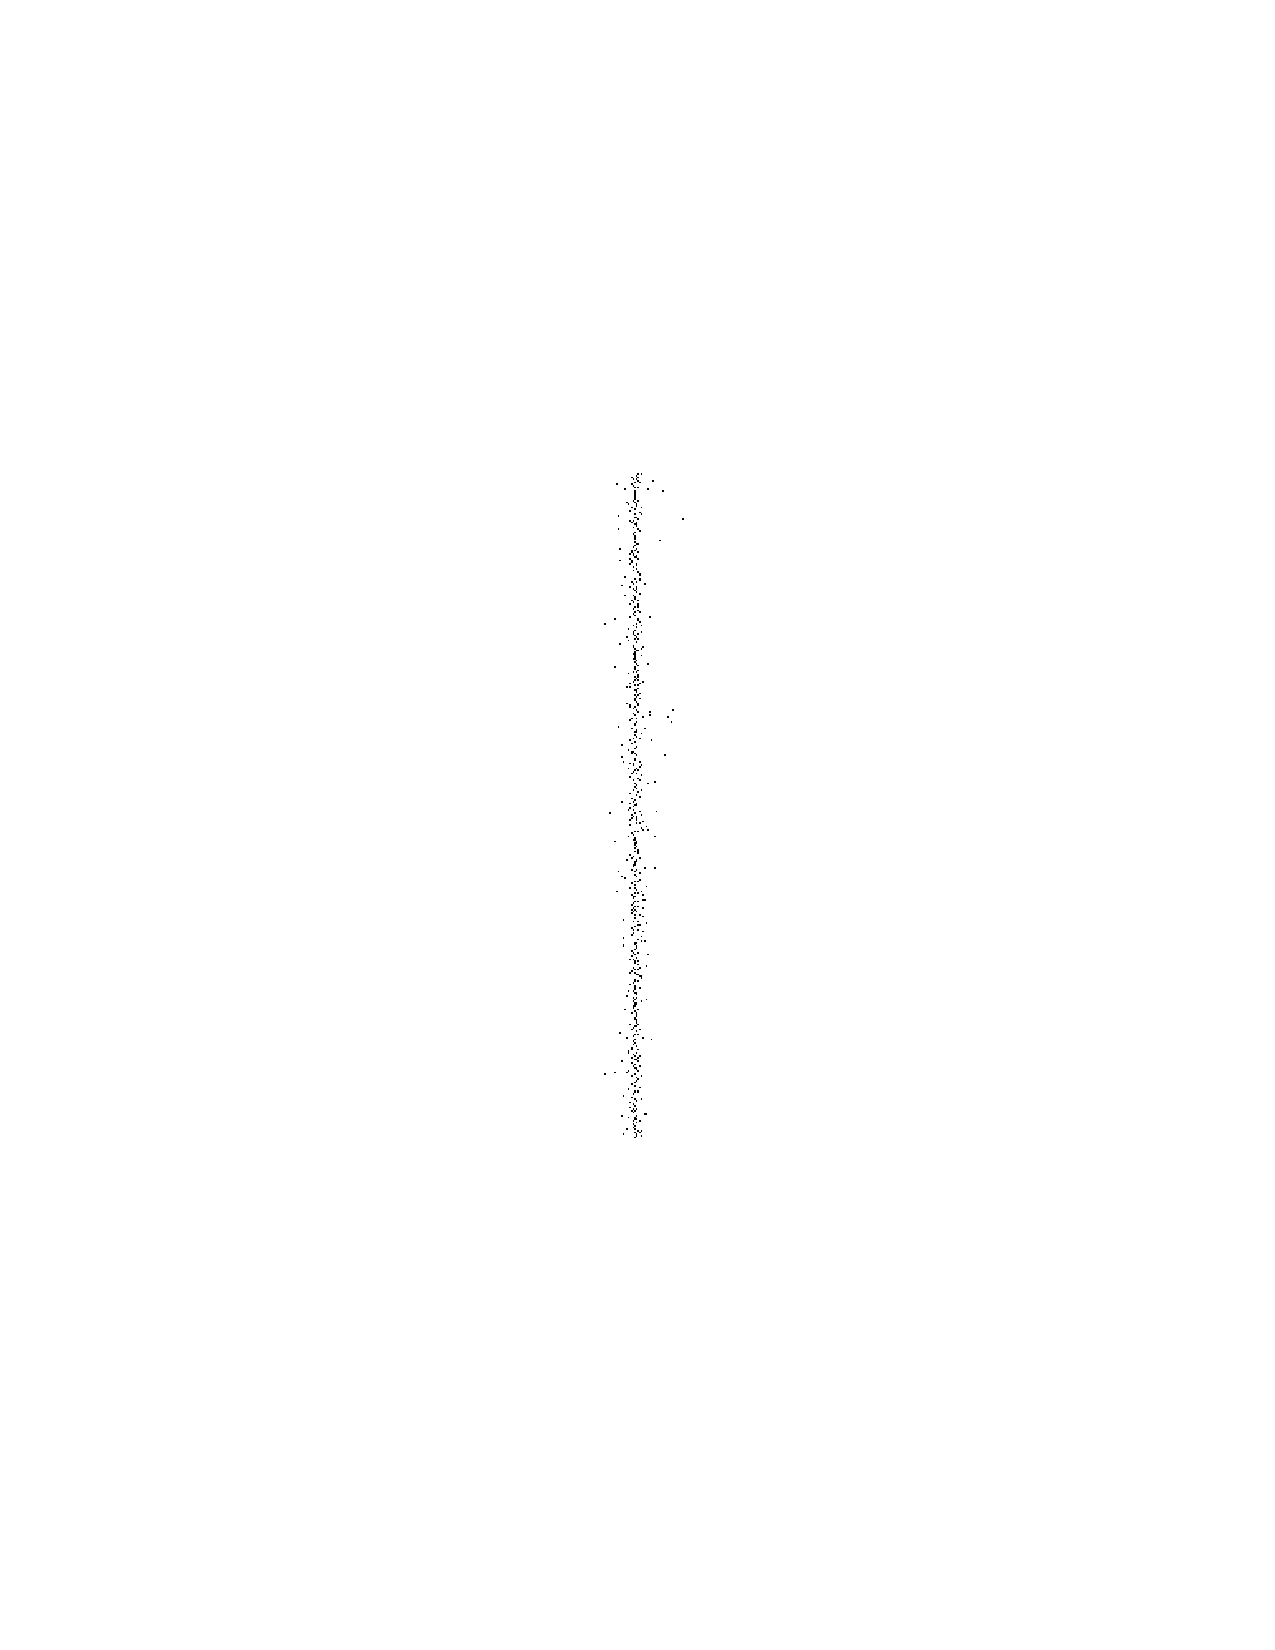
\includegraphics[width=\linewidth]{pca_fusao_hh_hv_vv_autovalor_1.pdf}}
\caption{Fusão com o menor autovalor $\lambda_1$}\label{cap_fusao_fig11}
\endminipage\hfill
\minipage{0.475\textwidth}
\fbox{ 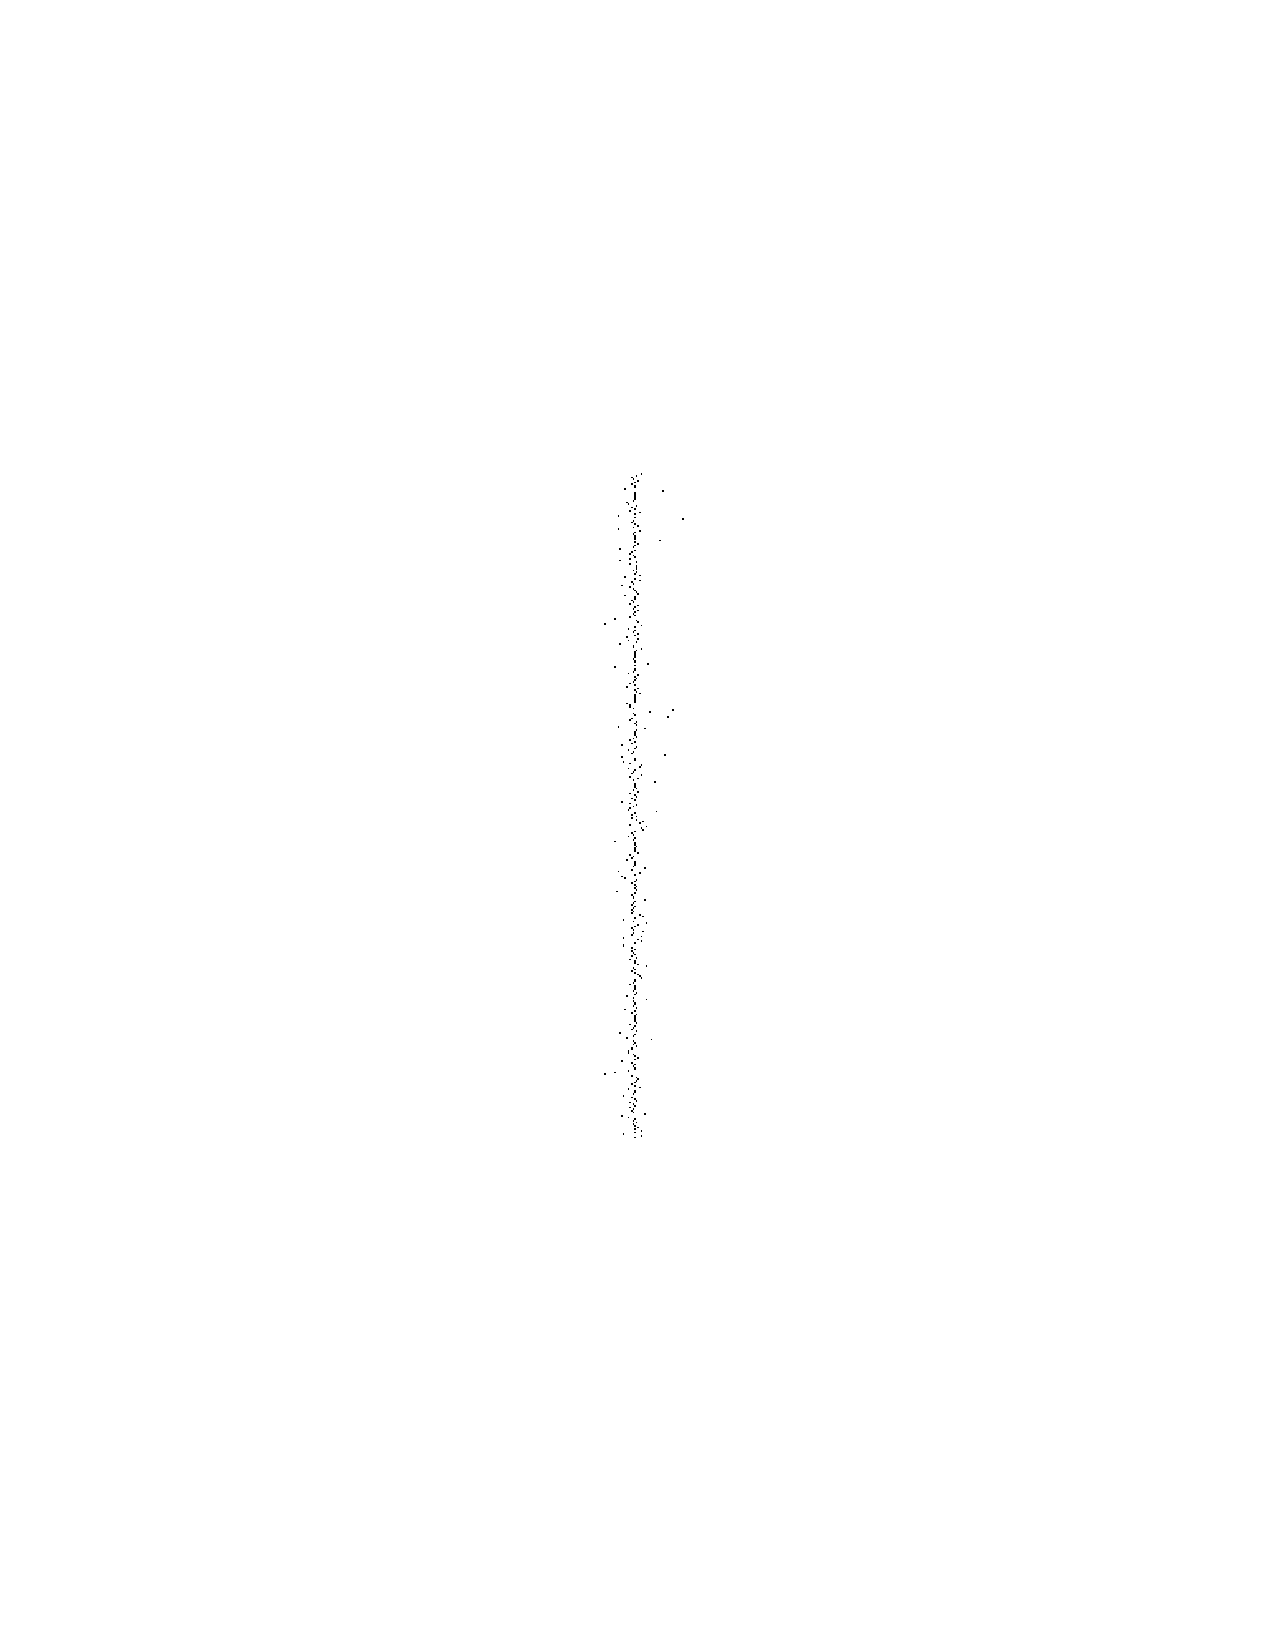
\includegraphics[width=\linewidth]{pca_fusao_hh_hv_vv_autovalor_2.pdf}}
\caption{Fusão com o autovalor $\lambda_2$}\label{cap_fusao_fig12}
\endminipage\hfill
\centering
\minipage{0.475\textwidth}
\fbox{ 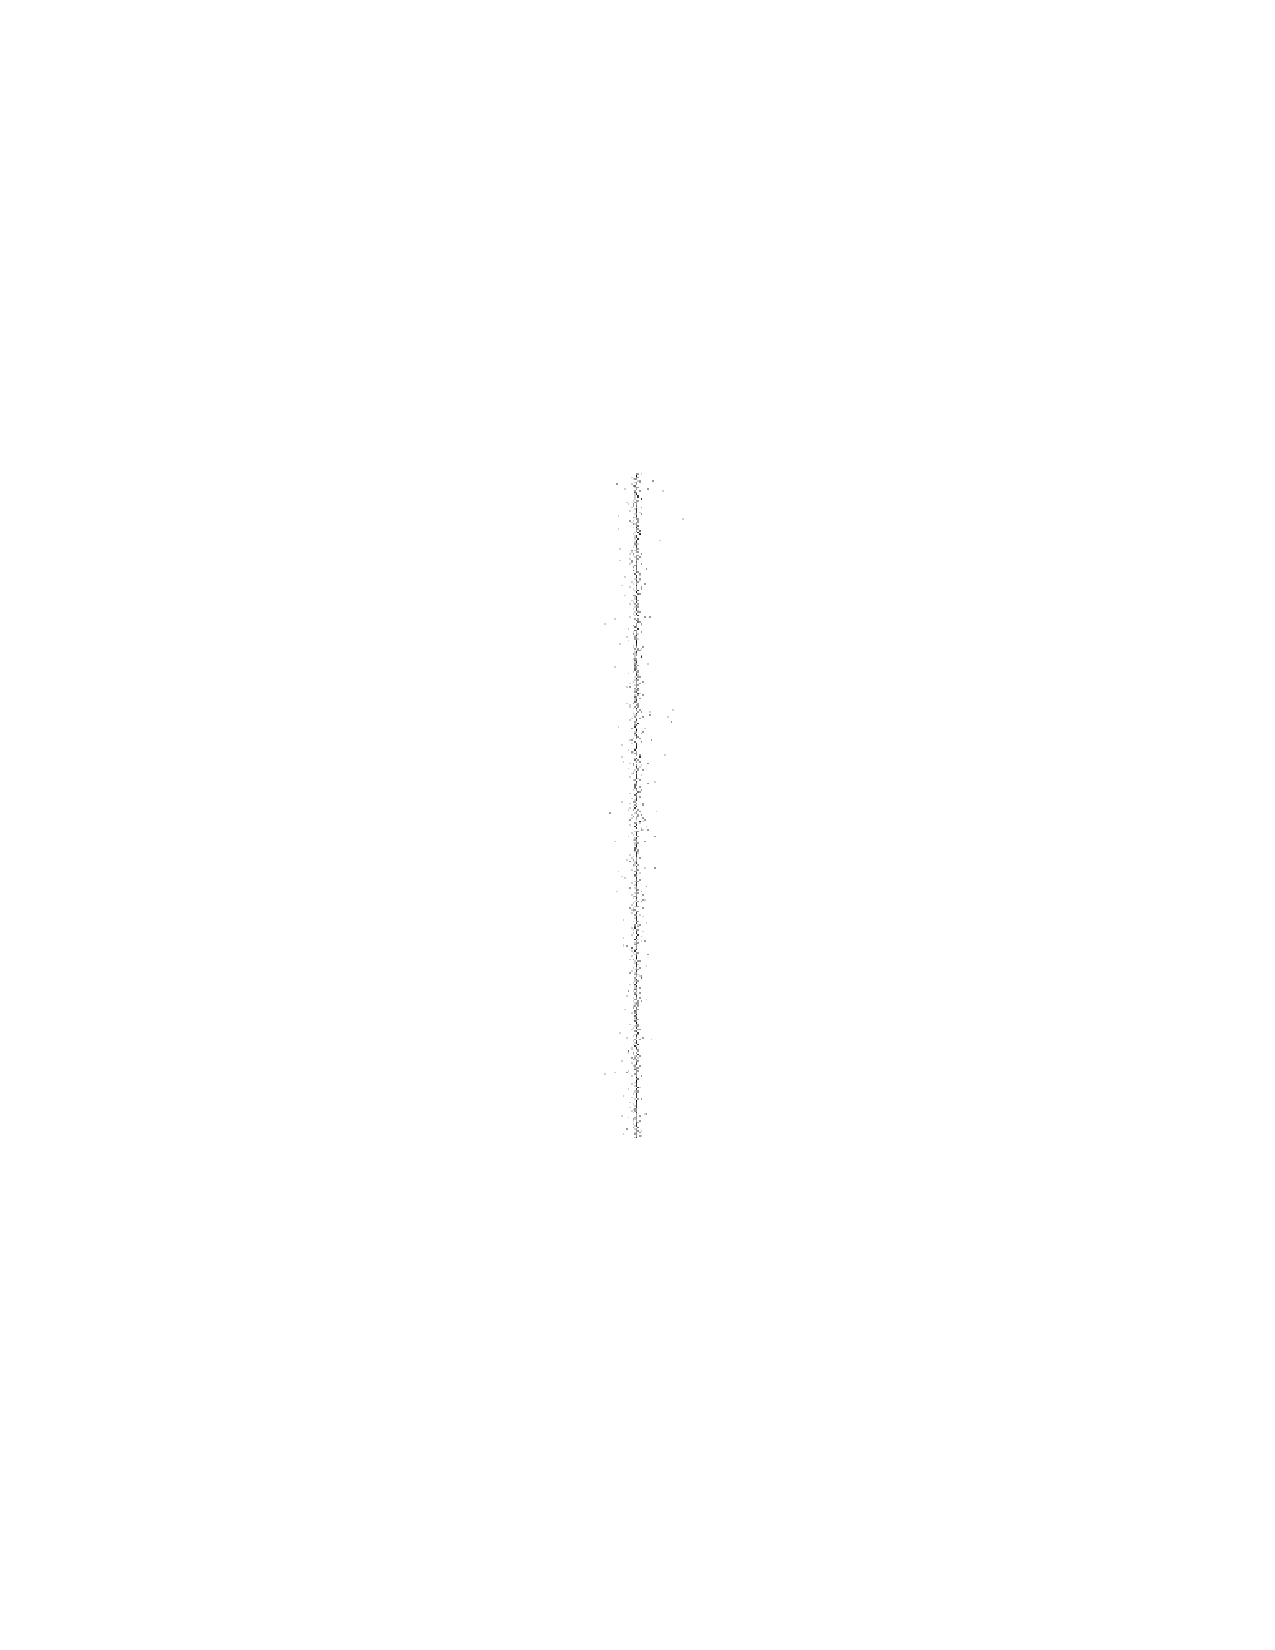
\includegraphics[width=\linewidth]{pca_fusao_hh_hv_vv_autovalor_3.pdf}}
\caption{Fusão com o maior autovalor $\lambda_3$}\label{cap_fusao_fig13}
\endminipage\hfill
\end{figure}

O método PCA aplicado nas imagens simuladas, 

\begin{figure}[!hbt]
\minipage{0.475\textwidth}
\fbox{  
\includegraphics[width=\linewidth]{pca_fusao_hh_hv_vv_autovalor_1_flor.pdf}}
\caption{Fusão com o menor autovalor $\lambda_1$}\label{cap_fusao_fig14}
\endminipage\hfill
\minipage{0.475\textwidth}
\fbox{ 
\includegraphics[width=\linewidth]{pca_fusao_hh_hv_vv_autovalor_2_flor.pdf}}
\caption{Fusão com o autovalor $\lambda_2$}\label{cap_fusao_fig15}
\endminipage\hfill
\centering
\minipage{0.475\textwidth}
\fbox{ 
\includegraphics[width=\linewidth]{pca_fusao_hh_hv_vv_autovalor_3_flor.pdf}}
\caption{Fusão com o maior autovalor $\lambda_3$}\label{cap_fusao_fig16}
\endminipage\hfill
\end{figure}
